\documentclass[12pt,a4paper]{report}

% ============================ 预加载的 LaTeX 包 ============================
\usepackage[a4paper,left=3.5cm,right=3cm,top=3cm,bottom=3cm]{geometry} % 页面边距
\usepackage[protrusion=true,expansion=false]{microtype} % XeTeX supports protrusion but not font expansion
\usepackage{setspace}                         % 设置 1.5 倍行距
\usepackage{fancyhdr}                         % 自定义页眉页脚
% amsmath/amsthm 须在 newtxmath 之前；勿加载 amssymb（与 newtxmath 的 AMS 符号重复）
\usepackage{amsmath,amsthm}                   % 数学与定理环境
\usepackage{newtxtext,newtxmath}              % Times New Roman 字体
\usepackage{graphicx}                         % 插入图片
\usepackage{hyperref}                         % 目录超链接
\hypersetup{hidelinks,colorlinks=false,linktoc=all}
\usepackage{booktabs}                         % 美化表格
\usepackage{array}                            % 处理表格对齐
\usepackage{multicol}                         % 多列布局
\usepackage[toc,page]{appendix}               % 处理附录
\usepackage{tocbibind}  % 让目录中包含“参考文献”和“附录”
\usepackage{caption}                          % 处理表格和图片标题格式
\usepackage{xcolor}                           % 颜色支持
\usepackage{titlesec}                         % 控制标题字体大小
\usepackage{eso-pic}                          % 添加水印
\usepackage{tikz}                             % 让水印精确定位
\usepackage{datetime}                         % 格式化日期
\usepackage{tocloft}                          % 目录格式控制
\usepackage{titletoc}                         % 目录格式增强
\usepackage{cite}                             % bib引用
\usepackage{longtable}                        % multi-page tables
\usepackage{tabularx}                         % width-aware tables
\usepackage{multirow}                         % grouped table entries
\usepackage{enumitem}                         % compact controlled lists
\usepackage{float}                            % stable figure placement
\usepackage{url}                              % software and dataset URLs
% \usepackage{showframe}
\usepackage{etoolbox}
\usepackage{ragged2e}
\usepackage[normalem]{ulem}                    % \uline 可断行，替代不可断行的 \underline
% Central metadata. Red fields require confirmation before submission.
\newcommand{\DissertationTitle}{Re-evaluating Released Vision-Language-Action Checkpoints on the RoboBenchMart Retail Benchmark: Octo and $\boldsymbol{\pi_{0.5}}$}
\newcommand{\AuthorName}{XU MAOKUAN}
\newcommand{\SchoolName}{School of Electrical and Electronic Engineering}
\newcommand{\ProgrammeName}{Signal Processing and Machine Learning}
\newcommand{\SubmissionYear}{2026}
\newcommand{\SupervisorName}{Yang Jianfei}


% ================================= 设置公式 ================================
\AtBeginEnvironment{equation}{\setstretch{1}}             % 设置公式1倍行距
\AtEndEnvironment{equation}{}                             % 公式结束恢复原样式
\numberwithin{equation}{chapter}                          % 让公式编号跟随章节
\renewcommand{\theequation}{\arabic{chapter}.\arabic{equation}}% 仅显示1.1

% ================================= 设置页脚 ================================
\pagestyle{fancy}                                         % 启用 fancyhdr
\fancyhf{}                                                % 清除默认的页眉和页脚
\fancyfoot[R]{\fontsize{12pt}{14pt}\selectfont \thepage}  % 右侧页脚页码 12pt
\renewcommand{\headrulewidth}{0pt}                        % 取消页眉下划线
\renewcommand{\footrulewidth}{0pt}                        % 取消页脚下划线
\fancypagestyle{plain}{                                   % 适配plain风格页面
    \fancyhf{} 
    \fancyfoot[R]{\fontsize{12pt}{14pt}\selectfont \thepage}
    \renewcommand{\headrulewidth}{0pt}
    \renewcommand{\footrulewidth}{0pt}
}

% ================================= 设置目录 ================================
% 修改目录标题格式（居中 + 18pt + 加粗 + 下划线）
\renewcommand{\contentsname}{}
\newcommand{\customtoc}{
    \clearpage
    \begin{center}
        \underline{\textbf{\fontsize{18pt}{18pt}\selectfont Table of Contents}}
    \end{center}
    \vspace{-1.2\baselineskip}
}
% 自定义 "Pages" 列标题，使其右对齐
\renewcommand{\cftaftertoctitle}{%
    \vspace{-1.5\baselineskip} % 减少 Table of Contents 后的额外空行
    \hfill\underline{Pages} % 右对齐
    \par\vskip-2\baselineskip % 调整间距，防止错位
}
%目录格式调整
% 一级标题 (chapter) 设置
\renewcommand{\cftchapfont}{\bfseries}                  % 章节标题加粗
\renewcommand\thechapter{\arabic{chapter}}                % 只用数字；\ref 也随之正常
\renewcommand\thesection{\arabic{chapter}.\arabic{section}}
\renewcommand{\cftchapaftersnumb}{}                     % 章节编号后不添加任何内容
\setlength{\cftchapnumwidth}{1.8em}                       % 编号宽度（只剩数字，收窄）
% 二级标题（section）设置
\renewcommand{\cftsecfont}{}                            % 节标题字体
\renewcommand{\cftsecpresnum}{}                         % 节编号前缀
\renewcommand{\cftsecaftersnumb}{}                      % 节编号后缀
\setlength{\cftsecindent}{0em}                          % 节的缩进
\setlength{\cftsecnumwidth}{2em}                        % 节编号宽度
\renewcommand{\cftsecdotsep}{\cftnodots}                % 移除点线
\renewcommand{\cftsecpagefont}{}                        % 节页码正常显示
% 间距设置
\setlength{\cftbeforechapskip}{0.5em}                   % 章节前的间距
\setlength{\cftbeforesecskip}{0.5em}                    % 节前的间距

% ========================== 统一设置 \chapter ==========================
% 设置有编号的 \chapter 显示 "Chapter 1" + 换行后的标题左对齐
\titleformat{\chapter}[hang]               % 章标题只显示标题名，不显示编号
  {\normalfont\Huge\bfseries}  % 不倾斜，字号 Huge，加粗
  {}                                       % 不输出章编号
  {0em}
  {\raggedright}
% 设置无编号的 \chapter*{}（如摘要、附录等）格式，不带 "Chapter"
\titleformat{name=\chapter,numberless}[display]
  {\normalfont\Huge\bfseries}  % 不倾斜，字号 Huge，加粗
  {}                                       % 无编号时不显示 "Chapter 1"
  {-2.5em}                                 % 章节编号和标题之间的间距
  {\centering}                             % 标题居中
% 调整章节标题的间距
\titlespacing{\chapter}{0pt}{-1em}{1.2\baselineskip}  % 影响有编号的章节
\titlespacing{name=\chapter,numberless}{0pt}{0em}{\baselineskip}  % 影响无编号的章节

% ========================== 统一设置 \section ==========================
% 设置有编号的 \section{}
\titleformat{\section}                        % 统一设置 section
  {\normalfont\fontsize{16pt}{16pt}\bfseries} % 12pt 字号行距，加粗
  {\thesection\enspace}                       % 章节编号（这里为空）
  {0pt}                                       % 章节前间距
  {\raggedright}                              % 章节后格式（这里保持默认）
% 设置无编号的 \section*{}
\titleformat{name=\section,numberless}[display]
  {\clearpage\normalfont\fontsize{16pt}{16pt}\bfseries}
  {}
  {-1em}
  {\centering}
\titlespacing{\section}{0pt}{0.5\baselineskip}{0.5\baselineskip}
\titlespacing{name=\section,numberless}{0pt}{0em}{1.5\baselineskip}

\global\sloppy  % 允许换行，减少溢出

% ======================= 统一设置 \subsection ========================
% 设置有编号的 \subsection{}
\titleformat{\subsection}    
  {\normalfont\fontsize{14pt}{14pt}\bfseries}  % 14pt 字号行距，加粗
  {\thesubsection\enspace}                     % 章节编号
  {0pt}                                        % 章节编号与标题间距
  {\raggedright}                               % 标题左对齐

% 调整 subsection 的间距
\titlespacing{\subsection}{0pt}{0.5\baselineskip}{0.5\baselineskip}


\begin{document}

\onehalfspacing % 1.5 倍行距

% ================================ 自定义颜色 ================================
\definecolor{DeepGreen}{rgb}{0.0, 0.690, 0.314}

% ================================ 自定义设置 ================================
% 左缩进为0
\setlength{\parindent}{2em}
% 自定义日期格式
\newdateformat{mydate}{\THEDAY\ \monthname[\THEMONTH]\ \THEYEAR}
% 让图编号显示为 "Figure X.Y"
\renewcommand{\thefigure}{Figure \arabic{chapter}.\arabic{figure}}
\setlength{\cftfignumwidth}{4.5em}
\renewcommand{\figurename}{}
% 图目录已移除（不再调用 \listoffigures）。如需恢复，取消下方注释并在前置部分加回调用。
% \makeatletter
% \renewcommand{\listoffigures}{%
%     \begingroup
%     \vspace{-2em}
%     \chapter*{\listfigurename}%
%     \@starttoc{lof}%
%     \endgroup
% }
% \makeatother
% 让表格编号显示为 "Table X.Y"
\renewcommand{\thetable}{Table \arabic{chapter}.\arabic{table}}
\setlength{\cfttabnumwidth}{4.5em}
\renewcommand{\tablename}{}
% 表目录已移除（不再调用 \listoftables）。如需恢复，取消下方注释并在前置部分加回调用。
% \makeatletter
% \renewcommand{\listoftables}{%
%     \begingroup
%     \vspace{-2em}
%     \chapter*{\listtablename}%
%     \@starttoc{lot}%
%     \endgroup
% }
% \makeatother


% ======================== 论文前置部分（Front Matter） =======================
\pagenumbering{gobble}
\begin{titlepage}
    \centering
    \vspace*{1cm}
    
\includegraphics[width=0.8\textwidth]{assets/ntu-logo-gray.png}
    \par                                  % 结束图片所在段落
    \vspace*{5.5cm}                       % 空白独立成段，不再插入标题内部
    % 长标题须整体排版，不可被垂直空白截断
    {\LARGE\bfseries \DissertationTitle\par}
    \vfill
    {\bfseries \AuthorName\par}
    \vspace{0.4cm}
    {\bfseries \MakeUppercase{\SchoolName}\par}
    \vspace{0.4cm}
    {\bfseries \SubmissionYear\par}

    \newpage
    \vspace*{4.5cm}
    \par\vspace*{0pt}                     % 确保下方标题从新段落开始
    {\LARGE\bfseries \DissertationTitle\par}
    \vspace*{4cm}
    \par
    {\bfseries \AuthorName\par}
    \vspace{1.5cm}
    {\bfseries \MakeUppercase{\SchoolName}\par}
    \vspace{1cm}
    {\bfseries A dissertation submitted in partial fulfilment of the requirements for the degree of
    Master of Science in \ProgrammeName\par}
    \vfill
    {\bfseries \SubmissionYear\par}
\end{titlepage}
             % 论文封面
\clearpage
\begingroup
\raggedright

\section*{\fontsize{14pt}{16pt}\selectfont Statement of Originality and Use of Artificial Intelligence Tools}

\vspace{0.4cm}

\begin{enumerate}[
  leftmargin=2.6em,
  labelsep=0.85em,
  itemindent=0pt,
  align=left,
  itemsep=1.15cm,
  topsep=0pt,
  parsep=0pt,
  partopsep=0pt
]
\setlength{\parskip}{0pt}
\setstretch{1.45}

\item I hereby certify that the work embodied in this thesis is the result of original research, is free of plagiarised materials, and has not been submitted for a higher degree to any other University or Institution.

\item I hereby declare that ChatGPT (OpenAI) was used to improve the clarity and readability of this thesis, and also to assist with drafting, structural revision, literature review and reference checking, and LaTeX preparation. I also declare that I have abided by NTU's \uline{Policy on the Use of GenAI in Research}, and I have reviewed and edited the content as needed after using this tool, and I take full responsibility for the content of this thesis.

\item All sources of information, ideas, data, and references used in this dissertation have been properly cited and acknowledged in accordance with the University's academic integrity policies.

\item I understand that any false declaration or breach of academic integrity may result in disciplinary action in accordance with the University's rules and regulations.

\item I acknowledge that the University reserves the right to verify this declaration and to take appropriate action should any violation be discovered.

\end{enumerate}

\vfill

\noindent
\begin{minipage}[b]{0.42\textwidth}
  \centering
  {\fontsize{13pt}{15pt}\selectfont 21/08/2026\par}
  \vspace{0.12cm}
  \rule{0.82\linewidth}{0.5pt}\par
  \vspace{0.15cm}
  Date
\end{minipage}
\hfill
\begin{minipage}[b]{0.42\textwidth}
  \centering
  \vspace*{0.9cm}
  \rule{0.82\linewidth}{0.5pt}\par
  \vspace{0.15cm}
  \AuthorName
\end{minipage}

\vspace*{0.45cm}
\endgroup
\clearpage
            % 原创性声明
\section*{Supervisor Declaration Statement}

\textcolor{red}{This page requires the supervisor's review and approved declaration wording. No supervisor approval, name, date, or signature has been inferred for this draft.}

\vspace*{1.5cm}
\begin{center}
\begin{tabular}{>{\centering\arraybackslash}p{6cm} p{1cm} >{\centering\arraybackslash}p{6cm}}
\textcolor{red}{DATE NOT PROVIDED} & & \SupervisorName \\
\dotfill & & \dotfill \\[0.2cm]
Date & & Supervisor
\end{tabular}
\end{center}
 % 导师声明
\section*{Authorship Attribution Statement}

This dissertation reports original research carried out by the candidate. The research design, implementation, experiments, analysis and dissertation writing are the candidate's own work. Third-party models, software libraries, datasets and published methods used in the study are acknowledged through the relevant citations and licence terms.

\vspace{0.5\baselineskip}

The candidate's contributions consist of the following work:

\begin{enumerate}[leftmargin=*,itemsep=0.15\baselineskip]
\item Development of a ManiSkill3-based simulation framework for retail mobile manipulation, including procedural scene generation and asset preparation.
\item Design and implementation of retail manipulation tasks and a shared pipeline for policy inference and evaluation.
\item Adaptation and experimental evaluation of vision-language-action policies within the developed framework.
\item Development of a demonstration collection and validation pipeline, and preparation of the dataset used in the study.
\item Analysis of experimental results and failure modes, together with verification and documentation of protocol discrepancies following a separate peer code review.
\end{enumerate}

\vspace{0.5\baselineskip}

All work claimed as a contribution in this dissertation was carried out by the candidate. Contributions originating from cited third parties are not claimed as the candidate's own work.

\vspace{0.5\baselineskip}



\vspace*{1.2cm}
\begin{center}
\begin{tabular}{>{\centering\arraybackslash}p{6cm} p{1cm} >{\centering\arraybackslash}p{6cm}}
21/08/2026 & & \AuthorName \\
\dotfill & & \dotfill \\[0.2cm]
Date & & Candidate
\end{tabular}
\end{center}
             % 著作声明

\clearpage
\centering\customtoc
\addtocontents{toc}{\protect\setcounter{tocdepth}{-1}} % 暂时隐藏目录
\tableofcontents % 生成目录
\addtocontents{toc}{\protect\setcounter{tocdepth}{1}}  % 恢复目录
\clearpage

\clearpage
\pagenumbering{roman}                         % 正文前使用罗马数字编号
\setcounter{page}{1}                          % 从 i 开始
\pagestyle{fancy}                             % 确保页码继续显示在右侧页脚
\chapter*{Abstract}
\addcontentsline{toc}{chapter}{Abstract}
\begingroup
\justifying
\setlength{\parindent}{2em}
\setlength{\parskip}{0.55\baselineskip}

Generalist robot policies are usually evaluated on tabletops or in household scenes. Retail dark stores pose a different problem: shelves are dense, products can look alike, and manipulation depends on precise local base positioning. This dissertation develops a ManiSkill3 project for studying that setting with loose products and articulated fixtures.

The project combines procedural store generation, configurable shelf population, motion-planning-based demonstration collection, and atomic and composite tasks. Collision-aware placement produces structured aisles, while serialised scene descriptions preserve evaluation conditions. In the recorded timing test, the original-mesh series ended at four shelving units; the simplified series included a 118-unit stocked scene. The policy study uses 2,976 successful demonstrations, comprising 1,401,169 transitions, to adapt Octo, SmolVLA, $\pi_0$, and $\pi_{0.5}$ across five atomic task families.

All adaptations ran on one NVIDIA RTX 4090 at batch size eight. Three used low-rank updates, every run stopped at a preset step count, and none used validation-based checkpoint selection. No policy exceeded 4\% success on any task under Pose; detailed cells ranged from zero to nine successes in one hundred trials. This floor-limited baseline, together with incomplete episode-level records, prevents design-aware Pose--Layout contrasts. The results describe four fixed-step pipelines, not the learning capacity of the underlying architectures.

A protocol audit, prompted by a separate code reading and reproduced by the author, narrowed the claim further. Nominally unseen products appeared on training shelves, four door tasks reused training scenes, and every episode began near the correct fixture. Conversely, policies acted open loop for fifty simulator steps and the torso remained fixed. Their net effect requires a rerun. The dissertation therefore offers an implemented and documented project, not a resolved policy ranking: visual plausibility was not measured, store-scale navigation was not tested, and retail-specific transfer remains open pending convergence-checked adaptation, matched conditions and complete episode records.

\endgroup
               % 摘要
\chapter*{Acknowledgements}
\addcontentsline{toc}{chapter}{Acknowledgements}

% ============================================================================
% 请用自己的措辞替换下方占位段落。建议顺序：
%   1) 导师  2) 其他学术/技术帮助  3) 机构与资助  4) 家人朋友
% 全篇 150-250 词为宜。写完后删除这些占位段落。
%
% 注意：本文正文字体为 Times New Roman，不含汉字，
%      占位文字必须用英文，否则 PDF 中会显示为空白。
%      AI 工具的使用披露属于原创性声明（originality.tex）的范围，不写在致谢里。
% ============================================================================

\textcolor{red}{[Paragraph 1 --- Supervisor. State specifically how \SupervisorName{} contributed, for example in shaping the research direction, reviewing the experimental design, or commenting on drafts. Avoid generic phrasing such as ``for his guidance and support''.]}

\vspace{0.5\baselineskip}

I am grateful to \textcolor{red}{[NAME]}, who read my experimental implementation against the protocol as this dissertation documents it and reported every place the two appeared to disagree. That review is the origin of the verification reported in Section~\ref{sec:verification}. Several of the discrepancies it surfaced were ones I had looked past repeatedly, and the account of the study is more accurate for them.

\vspace{0.5\baselineskip}

\textcolor{red}{[Paragraph 3 --- Institution: \SchoolName{}, Nanyang Technological University. Any scholarship or funding received must be acknowledged here.]}

\vspace{0.5\baselineskip}

\textcolor{red}{[Paragraph 4 --- Family and friends. One or two sentences are sufficient.]}
       % 致谢（内容待填写）
\input{c-front-matter/acronyms}               % 术语缩写表（可选）
\chapter*{Symbols}
\addcontentsline{toc}{chapter}{Symbols}

\noindent
\begin{tabular}{>{$}p{2.5cm}<{$}p{10cm}}
N, M & Store-floor dimensions in metres \\
p_i & Vertex of a polygonal boundary \\
u_i & Directed polygon edge vector \\
\theta & Local edge orientation \\
T_j(p) & Basis tensor associated with boundary sample $j$ \\
T(p) & Aggregated tensor field at point $p$ \\
d & Spatial decay coefficient in tensor-field aggregation \\
l & Length of a polygon edge \\
P & Number of vertices in a polygon \\
\end{tabular}
                % 符号表（可选）

% ========================= 论文正文部分（Main Content） ========================
\clearpage
\pagenumbering{arabic}       % 正文部分改为阿拉伯数字
\setcounter{page}{1}         % 从 1 开始
\pagestyle{fancy}            % 确保页码继续显示在右侧页脚
\chapter{Introduction}
\label{chap:introduction}
\begingroup
\justifying
\setlength{\parindent}{2em}
\setlength{\parskip}{0.55\baselineskip}

\section{Retail manipulation as a test for robot policies}

Moving a tin of beans from one shelf to the next sounds trivial. For a mobile robot it is a chain of small, unforgiving steps. The instruction names a product whose label may differ from its neighbour's only in a few words of type. The tin sits among other packages with a few centimetres to spare. The base has to stop where the arm can reach, and a stop that is a few centimetres short turns a grasp into a miss. Refrigerated fixtures add a different kind of difficulty: a door has to be found, contacted at the right place and moved through an arc while the base stays out of the way. Each of these problems is familiar on its own. A store puts them in the same aisle.

That combination makes retail an attractive setting for evaluating vision-language-action (VLA) policies, the family of models that map camera images and a written instruction directly to robot actions. Several such models are now public, together with recipes for fine-tuning them on new robots. Whether a released, fine-tuned checkpoint does what its authors report when someone else runs it is a separate question, and one that benchmark papers rarely answer for each other.

RoboBenchMart~\cite{soshin2025robobenchmart} is a recent benchmark for exactly this setting. Built on ManiSkill3~\cite{taomaniskill3}, it generates dark-store layouts procedurally, stocks them with a library of retail products, and defines pick-and-place and door tasks for a Fetch mobile manipulator. Its authors generated motion-planned demonstrations, fine-tuned four VLA policies on them, evaluated the policies under four increasingly demanding conditions, and released the code, the scenes and some of the fine-tuned checkpoints. That release is the starting point of this dissertation.

\section{Problem statement}

A benchmark result is only as useful as it is reproducible. In robot learning the gap between ``the code is public'' and ``the result can be reproduced'' is wide. A result depends on the policy weights, on the version of the simulator and the environment code, on how the policy is served and how its actions are applied, and on details of the evaluation protocol that a paper may summarise in a sentence. A change in any of these can change the outcome, and the changes are not always visible from the outside.

This dissertation asks a narrow version of that question for RoboBenchMart. If I take two of the released checkpoints, Octo and $\pi_{0.5}$, and run them through the benchmark's atomic evaluation protocol using only what is publicly available today, what results do I get? How do they compare with the published ones? And what can and cannot be concluded from the comparison? I did not train any model. I did not re-run the upstream study. I ran the released artefacts as released, recorded what happened, and examined the protocol closely enough to say what the numbers mean.

\section{Research questions}

\begin{description}[leftmargin=2.8em,style=nextline]
    \item[\textbf{RQ1}] Can the 42 atomic evaluation configurations of RoboBenchMart be run to completion using only the public code, scenes and checkpoints? What has to be repaired, and what evidence does the run leave behind?
    \item[\textbf{RQ2}] How many episodes does each checkpoint complete in each of the five task families under each condition, and which differences between conditions and between models can be resolved with 30 episodes per configuration?
    \item[\textbf{RQ3}] How far are these results from the upstream report, and how do properties of the protocol and differences between software versions limit the conclusions that can be drawn?
\end{description}

\section{Scope}

The study covers two policies, Octo~\cite{octo_2023} and $\pi_{0.5}$~\cite{intelligence2025pi05visionlanguageactionmodelopenworld}, as fine-tuned and released by the RoboBenchMart authors. Each was evaluated on the 42 atomic configurations defined in the benchmark's evaluation script: 12 under each of the Seeds, Pose and Layout conditions and 6 under Pairing, with 30 episodes per configuration. That is 1,260 episodes per model.

Several things are outside the scope, and it is worth listing them because the original benchmark covers them. I evaluated neither $\pi_0$ nor SmolVLA, both of which appear in the upstream paper. I ran no composite tasks. I did not annotate why episodes failed, so the upstream failure taxonomy is described but not applied. I did not fine-tune or train anything, and the training conditions of the checkpoints are known to me only from the upstream paper. All experiments are in simulation.

One further boundary turned out to matter more than I expected. The code and scenes I evaluated on are newer than the checkpoints. The environment has changed in several ways since the checkpoints were published, and I did not attempt to reconstruct the version the checkpoints were trained against. The results therefore describe the released checkpoints on the current release of the benchmark, and Chapter~\ref{chap:results} discusses what that implies.

\section{Contributions}

The contributions are modest and practical.

The main one is an independent, fully documented run of the RoboBenchMart atomic protocol for two released checkpoints: 2,520 episodes, each linked to a seed, a log line, a video and a SHA-256 hash, together with the revisions of every component involved.

Getting the protocol to run required three repairs, which I made and documented. The floor environments could not be constructed because an upstream change had removed an import still in use. The evaluation client read the instruction from a wrapped environment. And the Octo server shared one observation history across all connections, which would have mixed episodes once clients ran in parallel.

The results themselves are the third contribution. Neither checkpoint completed any of 1,800 pick-and-place episodes; $\pi_{0.5}$ closed doors in about a fifth of its attempts. This is far below the upstream figures, by a margin that sampling noise cannot account for.

Finally, I read the evaluation code closely enough to correct several statements about the protocol, including one I had made myself in an earlier draft: the evaluation client locks the robot's head, not its torso. I also identify the version changes between the checkpoints and the evaluated environment that are most likely to matter, and I propose a version-aligned re-evaluation as the direct test.

\section{Structure}

Chapter~\ref{chap:literature} reviews work on robot benchmarks, retail datasets, procedural environments, demonstration generation and VLA policies, and on the reproducibility of evaluation results. Chapter~\ref{chap:system} describes the RoboBenchMart benchmark, all of which is upstream work. Chapter~\ref{chap:methodology} describes how I evaluated the checkpoints, and Chapter~\ref{chap:results} reports and discusses the results. Chapter~\ref{chap:conclusion} draws conclusions and sets out the next experiments. The appendix lists every configuration's result, the component revisions and the records kept.

\endgroup
  % 第一章
\chapter{Literature Review}
\label{chap:literature}
\begingroup
\justifying
\setlength{\parindent}{2em}
\setlength{\parskip}{0.55\baselineskip}

\section{Why benchmark design matters}

A robot benchmark is sometimes treated as a collection of tasks plus a leaderboard. That description misses its scientific role. A useful benchmark specifies what changes, what remains fixed, how success is measured and which conclusions are licensed by the comparison. In robot learning, those choices are unusually consequential because the observation distribution, embodiment, controller and physical reset procedure can all change the apparent difficulty of a task.

Real-world evaluation has the strongest claim to operational relevance, but repeated trials are expensive and difficult to standardise. Objects wear, cameras move, human resetters differ and a failed manipulation can alter the next episode. Simulation trades some physical realism for repeatability, privileged state and rapid reset. It also makes counterfactual evaluation possible: the same policy can be tested with a new floor texture, a different store plan or a changed product split while other variables remain controlled. The trade is worthwhile only if the simulator preserves the geometric and interaction constraints that define the target domain.

Robot-learning suites occupy different points on this design spectrum. Meta-World and robosuite provide diverse tabletop tasks and modular control settings, while robomimic adds a systematic study of learning from offline human demonstrations~\cite{yu2020metaworld,zhu2020robosuite,mandlekar2021whatmatters}. ManiSkill2 broadens the range of embodiments, object models and manipulation families~\cite{gu2023maniskill2}. At room scale, iGibson 2.0 and Habitat 2.0 combine mobile manipulation with interactive household scenes and articulated objects~\cite{li2022igibson2,szot2021habitat2}. HomeRobot makes the integration problem explicit by evaluating navigation, novel-object grasping and placement in one open-vocabulary task~\cite{yenamandra2023homerobot}; ProcTHOR addresses a different bottleneck by generating large numbers of interactive training environments~\cite{deitke2022procthor}. Together, these systems show that task diversity, physical interaction and controlled generalisation can coexist. Their dominant settings are nevertheless tabletops and homes, not densely stocked stores.

Simulation also leaves a transfer question. RoboTHOR pairs simulated rooms with physical counterparts so that the drop between the two can be measured under aligned conditions, although its initial benchmark concerns embodied visual navigation rather than contact-rich retail manipulation~\cite{deitke2020robothor}. This distinction matters here: repeatable simulation is useful evidence, but it is not itself evidence of physical deployment.

The bias towards homes and tabletops is not superficial. Retail shelves contain repeated instances, near-duplicate packaging, tight clearances and fragile scene state. Fixtures create narrow aisles and long navigation distances. A policy may need to identify ``the Fanta bottle'' among visually adjacent branded products and then approach it from a pose compatible with the gripper. Household benchmark coverage therefore does not automatically imply retail competence. A dedicated benchmark is justified when the domain changes the distribution of geometry, appearance and failure, not simply when it supplies a new background texture.

\section{Retail datasets and the missing interaction layer}

Retail computer vision has produced substantial resources, but the datasets pose different problems. RPC records multi-product checkout scenes, whereas Products-10K concentrates on recognition among 10,000 fine-grained stock-keeping units~\cite{wei2019rpc,bai2020products10k}. The Grocery Store Dataset uses natural in-store images and a hierarchical label structure; the Freiburg Groceries Dataset supplies real-world grocery images at a coarser category level~\cite{klasson2019grocery,jund2016freiburg}. Across these resources, subtle packaging differences, clutter and domain shift make perception difficult. Their annotations still stop before physical action: they cannot determine whether a selected instance is reachable, whether the gripper collides with neighbouring stock or whether the object remains stable after placement.

Three-dimensional assets narrow part of this gap. Generic repositories such as YCB and ShapeNet have long supported manipulation and shape research~\cite{calli2015ycb,chang2015shapenet}; Google Scanned Objects adds more than a thousand simulation-ready scans of everyday items~\cite{francis2022gso}. Retail-specific collections better match product geometry and texture: IPA-3D1K contains reconstructed retail objects, while 3D-FRONT illustrates how textured assets and professionally designed layouts can be packaged as complete synthetic interiors~\cite{lindermayr2023ipa,fu2021threeDfront}. Access, licensing and scale remain practical constraints, and even a large mesh collection does not define a store. Assets still need consistent units, orientation, collision geometry and materials; they must then be placed on support surfaces, grouped like stock and simplified enough for interactive rendering.

Recent work begins to treat shelf picking as a generative robotics problem. FetchBot focuses on highly cluttered shelf arrangements, safety-aware retrieval and zero-shot transfer to a physical robot~\cite{liu2025fetchbot}. That focus is valuable, but an isolated shelf does not test movement through a store, variation in fixture layout or interaction with articulated refrigeration.

The closest neighbouring systems make the boundary sharper. FetchBench procedurally generates constrained fetching scenes---shelves, drawers, cabinets and baskets among them---and evaluates the full approach--grasp--retrieve chain with both modular and learned baselines~\cite{pmlr-v270-han25a}. It is deliberately object- and geometry-centred rather than retail-specific. Sari Sandbox moves in the other direction. It provides three virtual grocery-store layouts, more than 250 interactive products, an API-controlled embodied agent and SariBench human demonstrations for shopping tasks~\cite{gajo2025sari}. MarketGen generates complete supermarket environments from text or reference images, reports more than 1,100 goods and evaluates checkout unloading and in-aisle mobile manipulation with a sim-to-real study~\cite{hu2025marketgen}. RoboBenchMart, the benchmark used in this dissertation, pairs procedural dark-store layouts, stocked fixtures and motion-planned demonstrations in ManiSkill3, and reports fine-tuned VLA baselines under four evaluation conditions~\cite{soshin2025robobenchmart}. \ref{tab:retail-benchmark-comparison} summarises these systems without forcing them into a single ranking, and adds a row for the present study so that its narrower role is visible.

{\renewcommand{\arraystretch}{1.14}
\begin{table}[H]
\centering
\footnotesize
\begin{tabularx}{\textwidth}{
>{\RaggedRight\arraybackslash}p{0.16\textwidth}
>{\RaggedRight\arraybackslash}p{0.21\textwidth}
>{\RaggedRight\arraybackslash}X
>{\RaggedRight\arraybackslash}X}
\toprule
Resource & Scene and embodiment & Generated resources or data & Main evaluation emphasis \\
\midrule
FetchBench & Everyday fetching with a fixed-base Franka arm & Procedural shelves, drawers, cabinets and baskets; successful expert trajectories & Approaching, grasping and retrieving unknown objects in unseen constrained scenes \\
FetchBot & Densely cluttered shelves with a physical arm & Voxel-based simulated shelf scenes and an oracle-to-vision policy pipeline & Safety-aware retrieval and zero-shot sim-to-real transfer \\
Sari Sandbox / SariBench & Whole grocery stores with a VR avatar or API-driven agent & Three store layouts, 250+ interactive products and annotated human demonstrations & Navigation, inspection, manipulation, checkout and comparison with human behaviour \\
MarketGen & Complete supermarkets with cashier and mobile-manipulation agents & Agent-based procedural generation, 1,100+ goods and parameterised fixtures & Checkout unloading, in-aisle item collection and sim-to-real transfer \\
RoboBenchMart (upstream) & Dark-store retail with a Fetch mobile manipulator in ManiSkill3 & Procedural layouts, stocked fixtures, motion-planned demonstrations, fine-tuned checkpoints & Four VLA baselines under four conditions; atomic and composite tasks \\
This study & Same benchmark, current public release & No new data; 2,520 evaluation episodes with logs, videos and hashes & Independent re-evaluation of two released checkpoints and of the protocol itself \\
\bottomrule
\end{tabularx}
\caption{Scope comparison with adjacent retail and fetching systems. Counts and capabilities describe the cited releases; they are not normalised measures of benchmark scale or difficulty.}
\label{tab:retail-benchmark-comparison}
\end{table}}

The literature therefore suggests a layered gap. There is abundant 2D appearance data, a smaller number of 3D retail assets and even fewer systems that turn those assets into reproducible manipulation episodes. The missing layer is interaction: a task API, controller, success predicate and dataset path that let researchers move from ``which product is visible?'' to ``can the robot safely complete the requested operation?'' RoboBenchMart is an attempt to supply that layer. Whether its reported results can be recovered by an outside user is the question this dissertation takes up.

\section{Procedural environments and structured variation}

Procedural generation is attractive because a finite hand-built scene can be memorised. Randomness alone, however, is not enough. ProcTHOR uses procedural rules to scale interactive environments, Infinigen Indoors couples a constraint language with generated indoor assets, and Holodeck turns textual specifications into spatial constraints over retrieved assets~\cite{deitke2022procthor,raistrick2024infinigenindoors,yang2024holodeck}. Their mechanisms differ, but the shared lesson is simple: scene count matters only when generation also preserves structure. Uniformly scattering fixtures across a floor creates collisions, blocked aisles and arrangements that do not resemble stores.

RoboBenchMart's fixture placement draws on tensor-field methods for procedural street modelling~\cite{chen2008interactive}. In that setting, a field encodes locally preferred orientations; curves follow the field to form coherent road networks. A store presents a related geometric problem. Shelves usually align in rows, follow boundaries and leave passages between them. A second-order tensor is particularly useful because its principal directions are orientation-like: a shelf aligned at $0$ degrees is equivalent to one aligned at $180$ degrees. This symmetry avoids an arbitrary forward direction.

Several alternatives were possible. A fixed catalogue of plans would guarantee plausibility but provide limited continuous variation. Pure rejection sampling would diversify pose but struggle to produce coherent rows. Grammar-based layouts could encode strong design knowledge, although every new fixture relation would expand the grammar. A learned generator might capture examples from real plans but would require an appropriate corpus and a validity layer. The tensor-field approach occupies a practical middle ground: boundary and obstacle geometry induce local directions, while rejection tests still enforce collision and aisle constraints. Chapter~\ref{chap:system} shows how the upstream implementation actually uses the field, which is more discrete than the formulation suggests.

Procedural shelf population raises a different set of constraints. Products sit on detected support surfaces, typically in aligned groups. The \texttt{scene\_synthesizer} library provides scene and support-surface operations of this kind~\cite{eppner2025scene}. Visual diversity must also be accompanied by computational discipline. High-resolution product meshes multiply quickly, and a few hundred products per store can dominate memory and rendering time. Remeshing methods such as QuadriFlow~\cite{huang2018quadriflow} and simpler primitive approximations are the usual remedies; RoboBenchMart reports using simplified meshes for all but the nearest shelf~\cite{soshin2025robobenchmart}. This is an engineering optimisation rather than a learning contribution, yet it changes which experiments are feasible.

\section{Generating robot demonstrations}

Robot policy adaptation requires trajectories. Teleoperation gives human-like behaviour and can handle complex contact, but collection time grows with task and scene diversity. Physical teleoperation also carries reset cost. In simulation, privileged object poses and collision models make automatic collection possible. The central trade-off is between scalability and behavioural naturalness.

Sampling-based motion planning supplies collision-aware paths without learning a policy~\cite{LaValle_2006}. RRT-Connect grows two trees, one from the start and one from the goal configuration, for single-query planning~\cite{kuffner2000rrt}; OMPL packages this and other sampling-based algorithms behind reusable planning interfaces~\cite{sucan2012ompl}. Recent GPU systems take a different route: cuRobo combines parallel geometric search, inverse kinematics and trajectory optimisation for fast collision-free motion generation~\cite{sundaralingam2023curobo}. Asymptotically optimal sampling methods offer stronger theoretical properties at additional computational cost~\cite{KaramanSamplingBased}. For demonstration collection, however, the best planner is not necessarily the one with the strongest asymptotic guarantee. It is the one that produces enough successful, varied executions under a clear acceptance test.

RoboBenchMart's collector is of this pragmatic kind. Task logic defines waypoints for approach, grasp, transport and placement; between them, the planner first tries a screw motion~\cite{murray2017mathematical} and falls back to RRT-Connect when that fails. Only complete, successful episodes are kept. Such a scheme is scalable relative to manual demonstration, and seeded generation makes it reproducible in principle. It does not discover task structure automatically: waypoint design transfers human knowledge into the collector, and retaining only successes changes the trajectory distribution. The demonstrations show completion, but they do not teach recovery from error. Methods such as MimicGen take another route, transforming a small number of human source demonstrations across scenes and object poses~\cite{mandlekar2023mimicgen}. Reinforcement learning can generate behaviour through reward optimisation~\cite{sutton2018reinforcement,haarnoja2017soft}, yet reward design, exploration and computation remain substantial for long-horizon mobile manipulation. These families are complementary rather than mutually exclusive.

\section{Generalist vision-language-action policies}

Large heterogeneous robot datasets have encouraged policies that share representations across tasks and embodiments. Open X-Embodiment and DROID exemplify efforts to aggregate broad real-robot experience~\cite{open_x_embodiment_rt_x_2023,khazatsky2024droid}, addressing a data regime in which no single laboratory can cheaply collect every task and platform. Generalist policies then condition action generation on images, language and robot state.

Octo is a transformer-based generalist policy designed for adaptation across robots and tasks~\cite{octo_2023}. OpenVLA uses a vision-language backbone with autoregressive action prediction~\cite{kim24openvla}, Dita scales a diffusion transformer to the same problem~\cite{hou2025dita}, and the $\pi_0$ family pairs a vision-language foundation with a flow-based action component~\cite{black2024pi0visionlanguageactionflowmodel}. SmolVLA targets a smaller and more accessible model footprint~\cite{shukor2025smolvlavisionlanguageactionmodelaffordable}. $\pi_{0.5}$ extends the $\pi$ family toward open-world generalisation~\cite{intelligence2025pi05visionlanguageactionmodelopenworld}. These designs differ in scale, pretraining mixtures, action representation and adaptation recipe. A benchmark comparison therefore measures complete model pipelines, not model size in isolation.

Most of these models predict actions in chunks: a single inference returns several future actions, which are then executed before the policy is queried again. Chunking makes inference affordable and can smooth behaviour, but it also means that, for the length of a chunk, the policy cannot react to what it sees. How long a chunk is executed open loop is usually a deployment choice rather than a property of the model, and it is often reported only in passing.

Retail evaluation adds pressures that are less visible in a spacious tabletop setup. Grounding must discriminate branded instances in clutter. Manipulation needs centimetre-level alignment in constrained shelf cells. Mobile-base error changes the arm's reachable set. And when a task chains several stages, the probability of failure compounds.

The RoboBenchMart authors fully fine-tuned four of these models (Octo, SmolVLA, $\pi_0$ and $\pi_{0.5}$) on their demonstrations and released checkpoints for some of them~\cite{soshin2025robobenchmart}. Fine-tuning rather than zero-shot evaluation is appropriate for a domain-adaptation question, but it means each reported number belongs to a whole pipeline: pretrained weights, fine-tuning recipe, serving code and evaluation harness. When an outside user evaluates a released checkpoint, the first two parts are fixed and the last two are whatever the user's environment provides.

\section{Reproducibility of evaluation results}

Reproducibility problems in machine learning are well documented. In deep reinforcement learning, Henderson et al. showed that random seeds, implementation details and evaluation choices can change reported results by more than the differences between methods being compared~\cite{henderson2018deep}. The NeurIPS reproducibility programme responded with checklists and code-submission policies, while noting that sharing code is necessary but not sufficient~\cite{pineau2021improving}. Robot learning inherits these problems and adds its own: physical evaluation is costly to repeat, and simulated evaluation depends on simulator versions, assets and controller details that change over time.

Evaluating released policies in simulation has itself become a research topic. SimplerEnv, for example, builds simulated counterparts of real evaluation setups and checks whether policy rankings in simulation agree with those on hardware, paying explicit attention to control and visual mismatches between the two~\cite{li2024simplerenv}. The underlying lesson is that a policy checkpoint and an evaluation environment have to be matched carefully before their combination says anything about the policy.

Benchmark papers usually report results from a single evaluation infrastructure, maintained by the authors. Independent re-evaluations of the same released artefacts are rarer. I suspect one reason is that when the numbers do not match, the cause is hard to pin down after the fact, and an unexplained discrepancy is an awkward thing to publish. A re-evaluation is most useful when it records exactly what was run, so that a discrepancy can later be traced to a version, a configuration or a protocol detail rather than left as an unexplained gap.

\section{Generalisation, metrics and diagnostic evaluation}

Generalisation is meaningful only after its axis is named. A new robot pose tests local control robustness. A new texture tests visual invariance. A new floor plan changes navigation and camera geometry. An item that appeared in another task but not the current one tests whether the policy learned a transferable skill--object relation. A completely unseen object tests a stronger form of semantic and geometric transfer. Collapsing these cases into a single ``unseen'' score would hide useful structure.

The RoboBenchMart protocol defines a progression of this kind. Training-seed evaluation replays the configurations used for demonstrations; in-domain evaluation randomises the initial robot pose; unseen-scene evaluation changes the store; and unseen-scene-and-item evaluation pairs a familiar skill with an item not demonstrated for that task. The success rate is the primary metric,
\begin{equation}
    \widehat{S}_{m,t,c}=\frac{1}{N_{t,c}}\sum_{i=1}^{N_{t,c}} \mathbb{I}\!\left[\text{episode } i \text{ satisfies the task predicate}\right],
    \label{eq:success-rate}
\end{equation}
where $m$ denotes a model, $t$ a task, $c$ a condition and $N_{t,c}$ the number of episodes aggregated for that task and condition. The upstream study uses 100 episodes per task--item--fixture triplet. At that sample size, and more so at the 30 used here, the uncertainty in each rate is not negligible, and intervals rather than point estimates are the honest summary.

Success rates say how often a task is completed, not why it is not. The upstream authors address this with an eleven-category taxonomy that assigns each failed episode to the earliest stage at which it goes wrong. Choosing the earliest failure avoids double-counting cascades, at the price of hiding downstream damage, and the labels remain human judgements. A taxonomy of this kind needs per-episode evidence, ideally both video and state trajectories, to be applied consistently.

\section{Position of this dissertation}

This dissertation does not propose a model, a benchmark or a new evaluation condition. It takes one existing benchmark and two of its released checkpoints and asks whether the published results can be recovered from the public artefacts. Its contribution sits in the reproducibility layer described above: a complete, hashed record of what was run, a set of repairs needed to run it, and a careful reading of what the protocol does and does not measure. The benchmark design itself, including everything in Chapter~\ref{chap:system}, belongs to the RoboBenchMart authors.

\endgroup
  % 第二章
\chapter{System Design and Dataset}
\label{chap:system}
\begingroup
\justifying
\setlength{\parindent}{2em}
\setlength{\parskip}{0.55\baselineskip}

\section{Design requirements}

Evaluating mobile manipulation in a retail store seems deceptive at first glance. Position a mobile robot before a grocery display, prompt it to retrieve a box of cereal, and watch where execution falters. In simulation, that initial impression of simplicity evaporates almost immediately. Shelves pack hundreds of distinct meshes into narrow clearances. Refrigerator doors impose non-linear kinematic hinges. Mobile bases drift over long trajectories. Dense visual clutter easily overwhelms naive spatial representations. When an episode collapses, the failure must be diagnostic rather than opaque: we need to know whether the policy failed to ground the text prompt, misjudged the pre-grasp offset, lost friction mid-transport, or collided with an adjacent box.

Reproducing and verifying the RoboBenchMart benchmark~\cite{soshin2025robobenchmart} within ManiSkill3~\cite{taomaniskill3} required analyzing the entire system backwards from the demands of physical evaluation. A credible testbed must reconcile several competing engineering imperatives. Scenes must exhibit structural diversity without collapsing into geometric chaos: randomized floor plans must yield navigable aisles and physically plausible fixture alignments rather than arbitrary obstacle mazes. Generation must be strictly deterministic and inspectable, substituting stored, hash-indexed configuration files for unlogged chains of pseudorandom numbers. At the task boundary, success predicates cannot rely on simple bounding-box displacements; they must enforce rigorous collateral checks and stability conditions. Upstream demonstration synthesis must scale without demanding hundreds of hours of manual teleoperation. Finally, the policy interface must present a standardized observation--action contract capable of ingesting models as structurally divergent as diffusion transformers and autoregressive vision--language backbones.

These requirements crystallize into the five-layer decoupled architecture of the reproduced benchmark:
\begin{enumerate}[label=(\roman*),leftmargin=2.5em,itemsep=0.2em]
  \item \textbf{Scene Synthesis Layer}: Translates procedural store boundaries into collision-free fixture layouts and populated shelf inventories.
  \item \textbf{Simulation Environment Layer}: Instantiates the synthesized store within ManiSkill3, binds the Fetch mobile manipulator, configures lighting, and computes physical contacts.
  \item \textbf{Demonstration Generation Layer}: Leverages privileged simulator state, analytical kinematics, and motion planning to generate collision-free supervision trajectories.
  \item \textbf{Policy Evaluation Interface}: Exposes a multi-view visual and language-conditioned client, abstracting simulator specifics behind standardized sensor buffers.
  \item \textbf{Diagnostic Analysis Layer}: Evaluates terminal task predicates, monitors non-target disturbances, logs trajectory failures, and categorizes failure modalities.
\end{enumerate}

Decoupling these subsystems is an essential architectural decision. By isolating scene synthesis from policy rollouts, individual floor plans can be rendered, audited, and visually inspected long before any model consumes compute. Separating task predicates from learned controllers guarantees that ground-truth metrics remain strictly unpolluted by policy idiosyncrasies. Most critically, an identical library of frozen procedural seeds can be presented across every baseline architecture, ensuring that downstream performance variations reflect policy behavior rather than stochastic fluctuations in the environment.

\section{Store-plan generation}

A physical supermarket is not an unstructured scattering of furniture; it is an optimized topological network of parallel aisles, perimeter boundaries, and focal displays. To capture this spatial grammar procedurally, the generator models a store as a bounded two-dimensional polygonal floor plan $\Omega \subset \mathbb{R}^2$ populated by primary fixtures and structural obstacles. 

The generation pipeline executes in two successive passes. In the first pass, structural obstacles, structural columns, and large boundary fixtures are positioned via rejection sampling. Candidate footprints that intersect existing geometry or breach minimal clearance envelopes are discarded. This initial placement establishes the primary geometric contours that govern subsequent retail circulation.

The second pass synthesizes internal shelving runs by querying a continuous orientation field derived from boundary geometry. Let the store boundary and obstacle perimeters be represented by closed polygonal curves $\{\mathbf{p}_i\}_{i=1}^{P}$. Define directed edge vectors $\mathbf{u}_i = \mathbf{p}_{i+1} - \mathbf{p}_i$, with cyclic closure $\mathbf{p}_{P+1} = \mathbf{p}_1$. To prevent long wall segments from dominating local calculations, edges exceeding a threshold length $D$ are recursively subdivided. Each boundary segment, characterized by orientation $\theta_i = \operatorname{atan2}(u_{i,y}, u_{i,x})$ and length $\ell_i = \lVert\mathbf{u}_i\rVert_2$, induces an elementary symmetric traceless tensor:
\begin{equation}
  \mathbf{T}_i = \ell_i
  \begin{bmatrix}
  \cos(2\theta_i) & \sin(2\theta_i)\\
  \sin(2\theta_i) & -\cos(2\theta_i)
  \end{bmatrix}.
  \label{eq:basis-tensor}
\end{equation}
The doubled angle maps opposite directions to identical tensor representations, encoding an undirected axial orientation invariant to whether an edge is traversed clockwise or counterclockwise. For any floor query coordinate $\mathbf{x} \in \Omega$, the aggregated tensor field is computed via exponential distance decay:
\begin{equation}
  \mathbf{T}(\mathbf{x}) = \sum_i
  \exp\!\left(-d\,\lVert\mathbf{x}-\mathbf{p}_i\rVert_2\right)\mathbf{T}_i,
  \label{eq:tensor-field}
\end{equation}
where the decay parameter $d > 0$ determines the spatial decay rate of contour influence. The eigenvectors of $\mathbf{T}(\mathbf{x})$ define the locally dominant principal axes.

Because symmetry and tracelessness are preserved under linear combination, the accumulated tensor retains the canonical form:
\begin{equation}
  \mathbf{T}(\mathbf{x}) =
  \begin{bmatrix}
  a(\mathbf{x}) & b(\mathbf{x})\\
  b(\mathbf{x}) & -a(\mathbf{x})
  \end{bmatrix}.
\end{equation}
The dominant axial orientation $\theta^{\star}(\mathbf{x})$ is recovered analytically without full eigendecomposition:
\begin{equation}
  \theta^{\star}(\mathbf{x}) = \frac{1}{2}\operatorname{atan2}\!\left(b(\mathbf{x}),\,a(\mathbf{x})\right).
  \label{eq:tensor-orientation}
\end{equation}
This closed-form formulation reveals the underlying computational complexity. Evaluating Equation~\ref{eq:tensor-field} across $G$ floor query cells against $J$ discretized boundary samples scales as $\mathcal{O}(GJ)$ in time, with $\mathcal{O}(G)$ memory overhead. In a naive implementation, this cost scales directly with room perimeter and obstacle density. In the benchmark implementation, candidate queries are evaluated lazily along discrete sweep trajectories, avoiding exhaustive grid precomputation.

A minimal numerical example illuminates the tensor aggregation. Consider a horizontal boundary segment of length 2 passing directly through the query point ($\theta_H = 0$, $\ell_H = 2$, distance $0$), and an orthogonal vertical segment of length 1 located at a perpendicular distance of 1 unit ($\theta_V = \pi/2$, $\ell_V = 1$). Setting the decay parameter $d = 1$, their respective tensor contributions are:
\begin{equation}
  \mathbf{T}_{H} = 2
  \begin{bmatrix}1 & 0\\ 0 & -1\end{bmatrix},
  \qquad
  \mathbf{T}_{V} = e^{-1}
  \begin{bmatrix}-1 & 0\\ 0 & 1\end{bmatrix}.
\end{equation}
Summing these contributions yields:
\begin{equation}
  \mathbf{T}_{H} + \mathbf{T}_{V}
  = \begin{bmatrix}2 - e^{-1} & 0\\ 0 & -(2 - e^{-1})\end{bmatrix}
  \approx \begin{bmatrix}1.632 & 0\\ 0 & -1.632\end{bmatrix}.
\end{equation}
Applying Equation~\ref{eq:tensor-orientation} gives $b(\mathbf{x}) = 0$ and $a(\mathbf{x}) > 0$, producing $\theta^{\star} = 0^{\circ}$. The horizontal orientation dominates because the proximal, longer boundary outweighs the orthogonal segment.

In practice, the tensor field acts as a directional filter rather than a continuous protractor. Candidate fixtures are evaluated along orthogonal horizontal and vertical sweep vectors across the floor. Rather than rotating a shelf continuously to match $\theta^{\star}(\mathbf{x})$, the local orientation is tested against the Cartesian axes. If the principal direction falls within approximately $37^{\circ}$ of a coordinate axis, the candidate fixture is snapped to that axis. Consequently, every fixture in the synthesized store is strictly axis-aligned. The tensor field determines where an axis-aligned unit may reside, not its continuous heading. Candidate acceptance further demands an intersection-free footprint, compliance with a 2.0-meter passage envelope, and passage through an independent Bernoulli trial with a skip probability of $0.1$ to break rigid uniformity.

Moreover, the decay coefficient is configured to $d = 12$. At a radial distance of $r = 0.5$~meters, the exponential weight $\exp(-12 \times 0.5) \approx 0.0025$, collapsing the effective influence radius to approximately thirty centimeters. As a result, the orientation gate is almost entirely dictated by the single nearest boundary contour rather than a blended consensus of distant walls. The resulting floor plans achieve regular, well-separated aisle rows following perimeter geometries, but the underlying mechanism is an axis-snapped spatial gate rather than a continuous fluid field.

\begin{figure}[H]
    \centering
    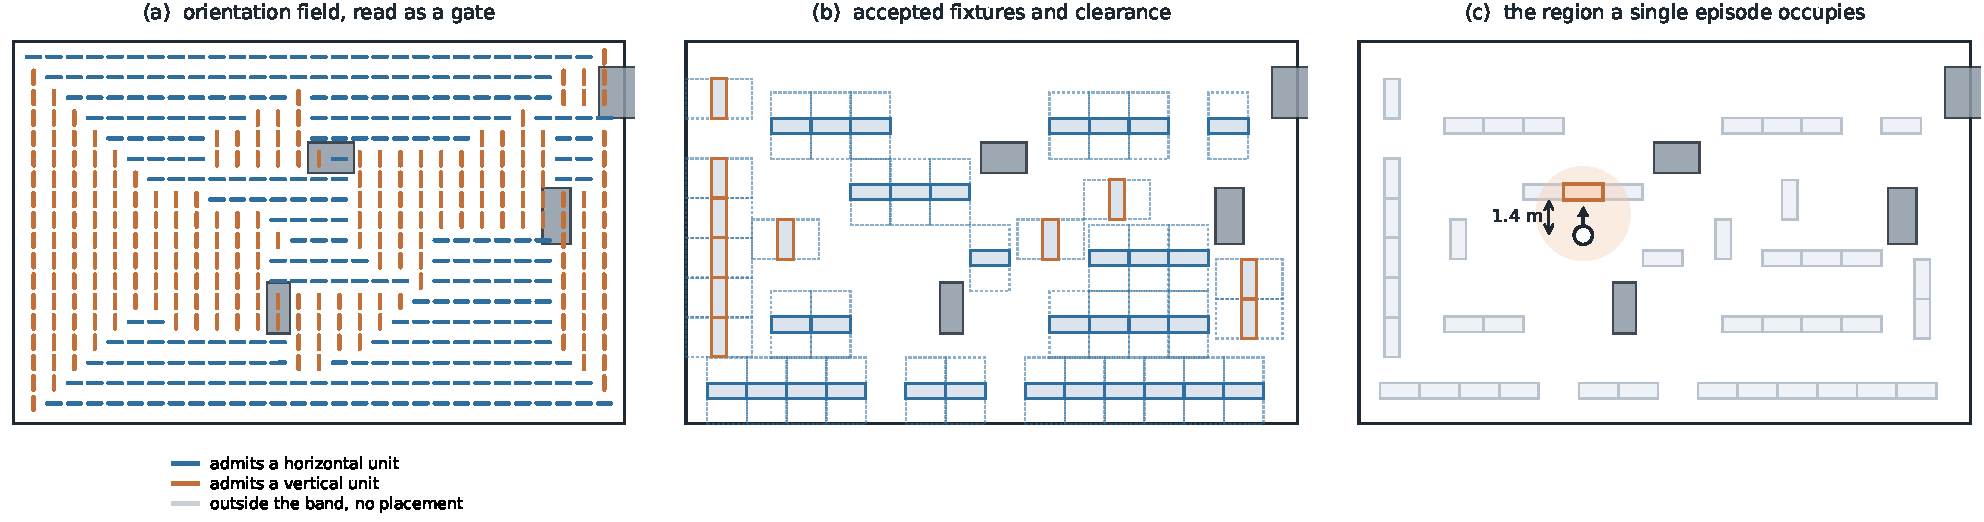
\includegraphics[width=\textwidth]{assets/figures/retail-vla-benchmark/layout_pipeline.pdf}
    \caption{Store generation pipeline for a $24\times15$~m retail space at $d=12$. (a) The discrete orientation field sampled across floor coordinates, displayed as unsigned axial ticks colored by acceptance gating. (b) Synthesized layout after collision, clearance, and passage rejection; units concatenate longitudinally to form multi-shelf runs. (c) Local episode footprint showing the active shelving unit, the robot's initial base placement at 1.4~m, and the operational workspace traversed during interaction. The simulation generates a multi-aisle supermarket, but policy execution remains confined to a local floor patch.}
    \label{fig:store-generation}
\end{figure}

\ref{fig:store-generation} illustrates the full synthesis progression. Panel (a) shows the orientation field sampled across a regular floor grid. Because the room boundaries are rectilinear, the field aligns with the coordinate axes across the vast majority of the interior. Rejection occurs primarily in regions where competing obstacle geometries induce diagonal vectors that fail the axial acceptance threshold. Panel (b) depicts the surviving store layout, demonstrating coherent multi-unit runs separated by generous aisles. Panel (c) highlights an important physical reality: while the generator synthesizes a comprehensive 360-square-meter supermarket, any single manipulation episode is restricted to a compact interaction envelope directly adjacent to an assigned fixture.

Standardized store environments measure $24 \times 15$~meters. Aisles maintain a minimum passage clearance of $2.0$~meters; free-standing shelving units maintain an occupancy buffer of $1.0$~meter, while wall-adjacent fixtures require $0.4$~meters. Boundary polygons are subdivided at $1.0$~meter intervals, and fixture perimeters at $0.5$~meters. If the procedural placement fails to satisfy valid scene constraints after twenty attempts, the seed is rejected.

Generated store definitions are serialized into compact JSON structures indexed by SHA-1 configuration hashes, enabling asynchronous batch production across multiple processor cores. The configuration schema specifies two distinct pseudorandom seed streams: one for structural floor layout and one for stock arrangement. In the evaluated benchmark configuration, both streams are initialized by adding the scene index to an identical base integer, locking layout and stock variation to the same underlying random sequence.

\section{Products, fixtures and visual variation}

The asset library comprises three commercial shelving units, two refrigerated merchandisers, and 371 retail product meshes spanning 21 retail categories, complemented by 23 legacy assets from preliminary design revisions. Surface materials are sampled from independent texture pools containing 26 floor, 17 wall, and 15 ceiling finishes. As shown in \ref{fig:asset-library}(a), asset distribution across categories is highly non-uniform: hygiene and spirits exceed forty distinct items each, whereas frozen commodities contain only two.

\begin{figure}[H]
    \centering
    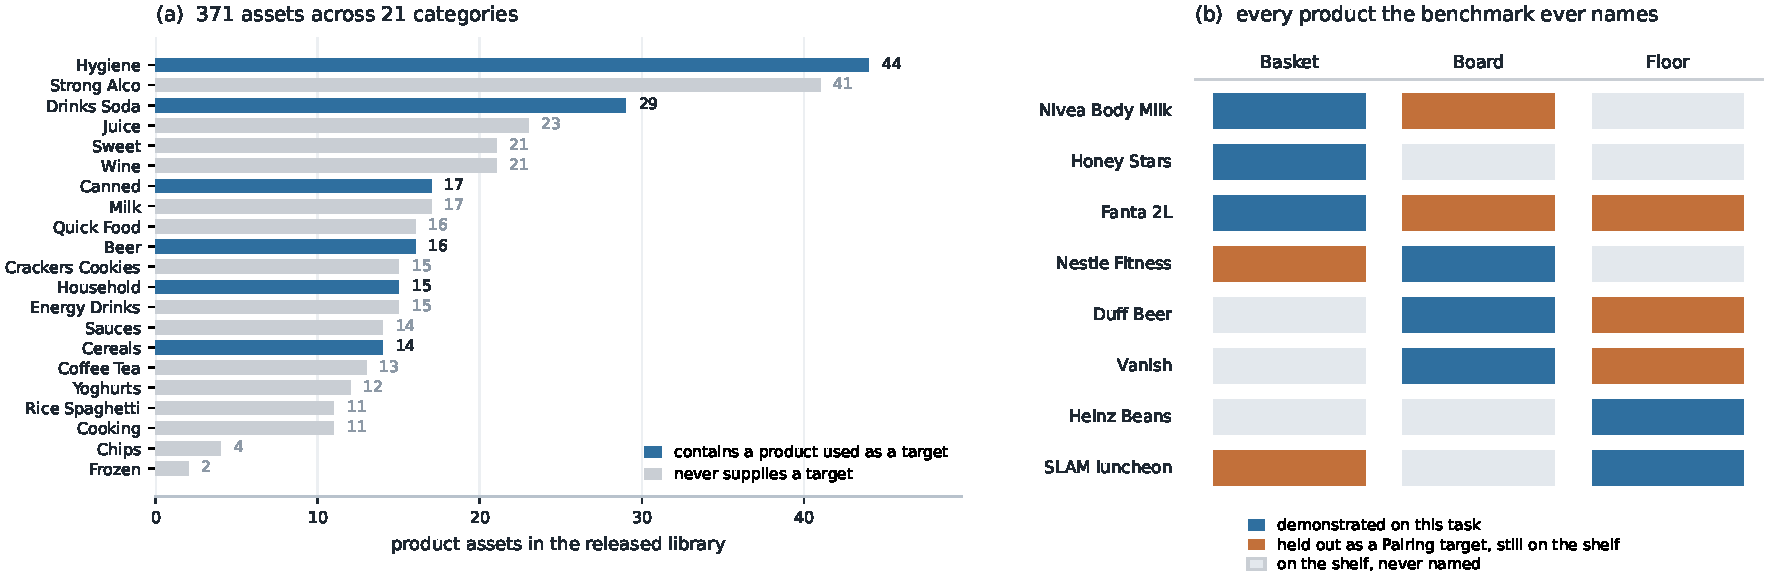
\includegraphics[width=\textwidth]{assets/figures/retail-vla-benchmark/asset_library.pdf}
    \caption{Asset catalogue distribution and evaluation coverage. (a) Total product assets per category across the 371-item catalogue; highlighted bars denote categories containing at least one task target. (b) The eight target products utilized in the evaluation benchmark and their roles across pick-and-place tasks. Crucially, products designated as unseen targets in the Pairing condition remain present as background clutter on training shelves throughout model adaptation.}
    \label{fig:asset-library}
\end{figure}

Panel (b) of \ref{fig:asset-library} reveals a critical boundary condition. Across the entire 371-item library, exactly eight products are ever referenced in task prompts. These eight items originate from six retail categories, and each serves as an interaction target in at most two distinct pick-and-place tasks. While the broader visual library is extensive, the empirical manipulation corridor is narrow. Claims regarding semantic grounding and zero-shot open-vocabulary generalization must be calibrated against this eight-object interaction set rather than the catalogue total.

Furthermore, \ref{fig:asset-library}(b) exposes an essential detail of the compositional evaluation split. A product withheld from task-specific training demonstrations is not absent from the visual world. It sits on the same shelves, rendered under identical lighting and camera perspectives, alongside active items during adaptation. The robot is repeatedly exposed to the visual geometry of these items; what is withheld is the pairing between the item's textual identity and the physical manipulation skill.

Integrating diverse third-party meshes into a rigid-body simulator introduces substantial physical friction. Raw assets sourced from heterogeneous 3D repositories exhibit incompatible dimensional units, non-standardized coordinate origins, and erratic bounding centers. Every asset underwent manual scaling against real-world retail packaging dimensions, orientation normalization, and support-surface annotation. Without accurate geometric scaling, gripper grasp envelopes and kinematic reachability checks become physically meaningless.

High-polygon meshes present an even steeper computational barrier. Retail packaging meshes frequently carry tens of thousands of triangles. Populating dozens of shelving units with unoptimized geometry instantly overwhelms GPU memory and collapses simulation throughput. To resolve this bottleneck, the benchmark deploys an automated mesh decimation pipeline incorporating QuadriFlow quadrangulation, Marching Cubes surface extraction, and primitive bounding proxies (boxes, cylinders). Candidate geometries are evaluated by measuring geometric deviation against the source mesh via Chamfer distance versus the remaining triangle budget.

\begin{figure}[H]
    \centering
    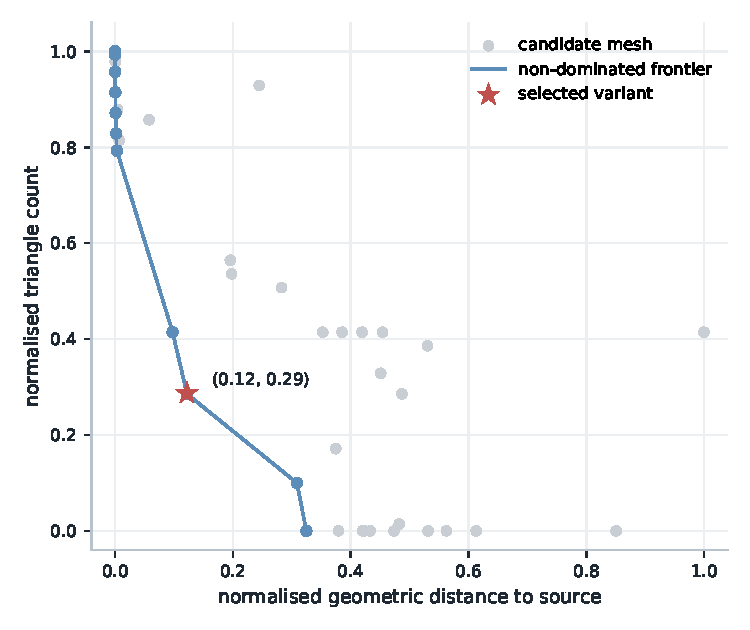
\includegraphics[width=0.62\textwidth]{assets/figures/retail-vla-benchmark/asset_pareto.pdf}
    \caption{Multi-objective mesh simplification Pareto frontier for a representative retail asset, normalized on both axes (lower is preferred). Out of 43 candidate approximations generated via QuadriFlow and decimation filters, eleven form the non-dominated Pareto frontier. A steep knee occurs at $(0.12,\,0.29)$, where triangle count drops by 71\% while preserving 88\% of source geometric fidelity.}
    \label{fig:asset-pareto}
\end{figure}

Selection cannot rely on a naive decimation ratio. As illustrated in \ref{fig:asset-pareto}, geometric error and polygon counts form a non-linear Pareto trade-off. Primitive geometric envelopes minimize polygon counts to negligible levels but obliterate distinctive product silhouettes, rendering visual grounding impossible. Conversely, aggressive remeshing algorithms occasionally increase triangle density without reducing Chamfer error. Across 43 evaluated simplification candidates, eleven reside on the non-dominated Pareto frontier. The optimal candidate was selected at the sharp knee of the curve, retaining 29\% of the original triangle count while incurring only 12\% of the maximum observed Chamfer error. Simplified proxies are deployed across all background fixtures, whereas foreground targets maintain high-fidelity collision envelopes.

Shelf population proceeds across identified horizontal support planes. Stock items are placed on a structured Cartesian grid subject to bounded translational and rotational perturbations ($\pm 1.5$~cm, $\pm 5^{\circ}$). This produces the dense visual arrangement characteristic of commercial grocery displays. While procedural mechanisms for vertical product stacking and Poisson-process stock depletion were formulated in initial design specifications, neither was deployed in the experimental environment. Every training and evaluation scene in this dissertation is fully packed.

\section{Robot and task environments}

Physical manipulation is simulated using the Fetch mobile manipulator in ManiSkill3~\cite{taomaniskill3}. The Fetch platform integrates a differential-drive mobile base for planar navigation, a prismatic torso joint providing vertical reach adjustment, a 7-degree-of-freedom articulated arm, and a two-finger parallel-jaw gripper. ManiSkill3 provides GPU-accelerated rigid-body dynamics, contact mechanics, and batch rendering.

The benchmark defines five canonical atomic tasks:
\begin{enumerate}[label=(\alph*),leftmargin=2.5em,itemsep=0.2em]
  \item \textbf{Pick to basket}: Locate a specified target product on a shelf or merchandiser, extract it from surrounding clutter, and deposit it into the robot's shopping basket.
  \item \textbf{Pick from floor}: Acquire a fallen target item resting on the floor surface and return it to a designated shelf tier.
  \item \textbf{From board to board}: Transfer an item from an upper or lower shelf tier to an alternate level within the same fixture.
  \item \textbf{Open fridge}: Grasp the handle of a refrigerated display door and articulate it past a specified angular opening threshold.
  \item \textbf{Close fridge}: Engage an open refrigerator door and push or swing it back into its fully latched position.
\end{enumerate}
In addition to standard refrigerator units, the codebase incorporates showcase merchandisers featuring four distinct articulated door leaves. These showcase variants share kinematic interaction mechanics with the primary refrigerator doors but specify discrete target handles, expanding the internal task registry beyond the five headline atomic families.

Natural-language prompts specify the target product and fixture description without exposing simulator entity pointers (e.g., \texttt{"pick the green tea box from the second shelf and place it in the basket"}). If duplicate candidate fixtures exist within the store, the policy is expected to navigate to and interact with the closest instance. This structure mirrors human operational instructions while requiring the model to resolve physical grounding autonomously.

Task success predicates enforce strict spatial and kinematic constraints rather than superficial target displacement:
\begin{equation}
  y = \mathbb{I}[o^* \in G]\;\mathbb{I}[\lVert\mathbf{v}_{\text{robot}}\rVert_2 \leq v_{\text{tol}}]\;\prod_{o \in \mathcal{N}(o^*)} \mathbb{I}[\lVert\Delta \mathbf{p}_o\rVert_{\infty} \le \epsilon_p \;\land\; \lVert\Delta \mathbf{q}_o\rVert_{\infty} \le \epsilon_q].
  \label{eq:predicate-success}
\end{equation}
For pick-and-place tasks, the target item $o^*$ must settle within the designated target volume $G$, the robot platform must come to a complete rest ($\lVert\mathbf{v}_{\text{robot}}\rVert_2 \leq 0.2$~m/s), and surrounding collateral objects $\mathcal{N}(o^*)$ must remain undisturbed within translational ($\epsilon_p = 0.1$~m) and rotational ($\epsilon_q = 0.1$) tolerances. In the basket task, $G$ is defined as a $0.4\times 0.4\times 0.4$~m bounding box centered on the onboard basket (expanded to $0.5$~m for large cereal packaging such as Honey Stars), and non-target monitoring is restricted to the active fixture shelf. For board transfer, $G$ specifies a $0.1$-meter horizontal boundary centered $0.397$~meters above the source shelf. For door tasks, success hinges on articulation metrics: showcase doors must reach $1.57 \pm 0.2$~radians (or return to $0 \pm 0.2$~rad for closure), whereas refrigerator covers require reaching $0.624 \pm 0.1$~radians (approximately $35.8^{\circ}$).

Two composite tasks are defined within the upstream RoboBenchMart benchmark to evaluate sequential horizon scaling:
\begin{itemize}[leftmargin=2.5em,itemsep=0.2em]
  \item \textbf{Pick three items}: Sequentially locate, grasp, and deposit three distinct target products into the mobile basket across successive prompt instructions.
  \item \textbf{Pick from fridge}: Execute a three-stage sequential chain: open the refrigerator door, extract the internal target beverage into the basket, and close the door.
\end{itemize}
In the upstream design, an algorithmic oracle monitors the subtask predicate and issues the subsequent natural-language prompt upon verified completion of the preceding stage. While these multi-stage tasks provide a conceptual framework for long-horizon planning, the empirical campaign in this dissertation restricts its scope strictly to atomic primitives, where baseline physical execution can be rigorously isolated and measured.

\section{Training corpus and demonstration provenance}

In the upstream RoboBenchMart framework, supervised training demonstrations were generated algorithmically across twelve canonical task--item--fixture configurations. The upstream collection pipeline captured 248 verified trajectories per triplet, yielding a nominal corpus of 2,976 demonstration episodes and 1,401,169 state--action transitions. In our reproduction environment, the repository preserves the twelve configuration index files and 2,976 episode metadata headers defining these trajectories. However, because local data containers store configuration metadata rather than full continuous state--action sensor arrays, this dissertation does not claim to have generated or trained on a local 1.4-million transition dataset. Instead, this metadata documents the training distribution of the publicly released fine-tuned checkpoints evaluated in Chapter~\ref{chap:results}.

Each transition records three complementary sensory streams:
\begin{itemize}[leftmargin=2.5em,itemsep=0.2em]
  \item \textbf{Language Prompt}: A descriptive task instruction specifying target product and destination fixture.
  \item \textbf{Visual Observations}: Three synchronized RGB camera views, consisting of exterior left-shoulder ($256\times 256\times 3$), exterior right-shoulder ($256\times 256\times 3$), and an eye-in-hand wrist camera ($128\times 128\times 3$). The robot's native head camera was omitted because the Fetch arm frequently blocks its line of sight during close manipulation.
  \item \textbf{Proprioception}: Joint positions and velocities of the 7-DOF arm, parallel gripper, and mobile base.
\end{itemize}

The commanded action is structured as a 13-dimensional continuous vector:
\begin{equation}
  \mathbf{a}_t = \left[\mathbf{q}^{\text{arm}}_t,\ a^{\text{grip}}_t,\ \mathbf{q}^{\text{body}}_t,\ v^{\text{base}}_t,\ \omega^{\text{base}}_t\right] \in \mathbb{R}^{13},
  \label{eq:action-vector}
\end{equation}
comprising seven arm joint target angles $\mathbf{q}^{\text{arm}}_t \in \mathbb{R}^7$, a scalar gripper position command $a^{\text{grip}}_t \in [0, 1]$, three body joint targets $\mathbf{q}^{\text{body}}_t = [q_{\text{torso}}, q_{\text{pan}}, q_{\text{tilt}}] \in \mathbb{R}^3$, and planar base linear and angular velocities $(v^{\text{base}}_t, \omega^{\text{base}}_t)$. Arm and torso joints operate under a proportional-derivative position-target controller, while the mobile base is governed by velocity setpoints.

A critical physical constraint was discovered during our runtime protocol audit. In the experimental evaluation client, the torso-lift and head-pan command dimensions are explicitly overwritten with zero at every simulation step. Because the low-level controller interprets joint setpoints as absolute coordinates rather than incremental displacements, this zero-clamping forces the prismatic torso to remain permanently pinned at its mechanical minimum ($q_{\text{torso}} = 0$). Demonstrations collected by the motion planner were likewise initialized and executed with the torso at zero. Consequently, across every policy, task, and demonstration in this benchmark, the robot operates with an entirely rigid spine. Vertical reach is a frozen constant of the environment, fundamentally constraining the robot's physical reach during floor retrieval and upper-shelf placement.

\section{Design decisions and rejected alternatives}

The technical design of this benchmark reflects deliberate engineering compromises between physical fidelity, computational throughput, and diagnostic clarity.

\textbf{Procedural Stores versus Isolated Shelf Cells.} An alternative approach would decouple manipulation from store environments, evaluating policies exclusively on isolated single-shelf modules. While an isolated shelf reduces rendering overhead and accelerates reset cycles, it destroys the visual and geometric context essential for embodied agents. Whole-store procedural generation forces the policy to operate under realistic visual backgrounds, varying aisle perspectives, and realistic global lighting, while preserving layout coherence for future navigation benchmarks.

\textbf{Serialized Plans versus Online Generation.} Rather than generating floor plans procedurally inside the environment reset loop, layouts are pre-synthesized, verified, and serialized into static JSON configuration files. This separation enables rigorous experimental version control: every model baseline is evaluated against the exact same frozen geometry and initial object poses. Furthermore, failed rollouts can be re-rendered and debugged offline without re-running stochastic generation routines.

\textbf{Continuous Fields versus Discrete Orientation Sweeps.} The theoretical formulation of Equations~\ref{eq:basis-tensor}--\ref{eq:tensor-orientation} allows continuous orientation interpolation. However, continuous shelf angles in a rectilinear retail store produce awkward triangular dead spaces and irregular aisles that fail standard accessibility constraints. The benchmark design therefore restricts the tensor field to act as an acceptance gate along Cartesian sweep vectors, preserving realistic aisle geometries while retaining boundary sensitivity.

\ref{tab:layout-generation-ab} summarizes the analytical trade-offs governing the layout synthesis architecture.

{\renewcommand{\arraystretch}{1.18}
\begin{table}[H]
\centering
\footnotesize
\begin{tabularx}{\textwidth}{
>{\RaggedRight\arraybackslash}p{0.18\textwidth}
>{\RaggedRight\arraybackslash}X
>{\RaggedRight\arraybackslash}X
>{\RaggedRight\arraybackslash}X}
\toprule
Dimension & Handcrafted templates & Unconstrained random placement & Tensor-gated sweep (RoboBenchMart suite) \\
\midrule
Source of order & Static human architectural designs & Independent random coordinates; order emerges only by rare chance & Boundary contours induce continuous axial orientation fields \\
Layout diversity & Restricted to manual permutations and minor parametric offsets & High, but frequently geometrically degenerate & Continuous procedural variation across seeds while preserving aisle corridors \\
Clearance enforcement & Hardcoded during authoring; easily invalidated by scaling & Enforced through brute-force rejection sampling & Rejection sampling guided by directional clearance envelopes \\
Boundary adaptation & Requires bespoke repair scripts for non-rectangular rooms & Geometrically flexible, but generates irregular, disjoint pockets & Automatically aligns runs with non-standard perimeter geometry \\
Computational profile & Negligible runtime; substantial human authoring burden & Inexpensive proposals; rejection rate surges under high spatial packing & $\mathcal{O}(J)$ field evaluations per candidate; easily parallelized across cores \\
Characteristic flaws & Rigid visual repetition; poor coverage of novel layouts & Chaotic fixture angles; unnavigable dead ends; floating geometry & Sensitive to decay parameter $d$, grid stride, and skip probability \\
Unaddressed constraints & Operational logistics, fire codes, and dynamic restock routes & Retail semantics, product adjacency, and physical accessibility & Customer traffic flow, inventory clustering, and operational zoning \\
\bottomrule
\end{tabularx}
\caption{Analytical design comparison of store-layout synthesis paradigms.}
\label{tab:layout-generation-ab}
\end{table}}

\textbf{Sensor Configuration.} The Fetch robot's default head camera was deliberately replaced with bilateral shoulder-mounted cameras and a wrist-mounted eye-in-hand sensor. In empirical manipulation rollouts, the Fetch arm routinely passes directly in front of the head mast, occluding the target item during critical grasping phases. The dual shoulder setup maintains an unobstructed global view of the fixture and surrounding stock, while the wrist camera supplies high-resolution local feedback during final contact closure.

\textbf{Algorithmic Planning versus Human Teleoperation.} Generating 2,976 demonstrations via human teleoperation would require hundreds of hours of manual labor and introduce substantial operator-dependent trajectory jitter. Algorithmic motion planning combining screw interpolation and RRT-Connect fallback guarantees repeatable, collision-free demonstrations at scale. The trade-off is clear: algorithmic planners generate clean, nominal trajectories that lack natural human recovery behaviors, an empirical constraint explored thoroughly in our failure analysis.

\section{Implemented scope}

To maintain rigorous scientific clarity, we explicitly distinguish between capabilities formulated in system specifications and the physical features exercised in the empirical evaluation. Stock depletion mechanisms and vertical box stacking were specified during pipeline design, but neither was deployed during experimental data collection or policy evaluation. Every shelf in this dissertation is fully populated to maximum capacity. Holding shelf density constant eliminates one uncontrolled source of variance, ensuring that baseline differences reflect layout geometry, viewpoint, and product identity rather than fluctuating occlusion levels.

Similarly, the mesh simplification frontier documented in \ref{fig:asset-pareto} represents a preprocessing intervention. Stepping an unoptimized 118-unit store scene choked simulation frame rates beyond four units; deploying simplified meshes enabled stable execution across large environments on a single GPU. These engineering constraints define the concrete operational testbed upon which the empirical methodology of Chapter~\ref{chap:methodology} is constructed.

\endgroup
  % 第三章
\chapter{Methodology}
\label{chap:methodology}
\begingroup
\justifying
\setlength{\parindent}{2em}
\setlength{\parskip}{0.55\baselineskip}

\section{Experimental logic}

The methodology links the three research questions to observable evidence. RQ1 requires generated plans that can be simulated and navigated, plus qualitative and performance evidence that dense scenes remain usable. RQ2 requires a documented path from task specification to successful demonstrations and a stable policy interface. RQ3 requires controlled splits, repeated trials and failure labels. No single number answers all three.

The experimental unit is a policy episode in a generated store environment. An episode is defined by a task, named target, fixture context, environment seed and evaluation scenario. The policy receives only language, RGB observations and proprioception through its adapter. Ground-truth object and fixture state remain inside the simulator for resetting and success evaluation. Demonstration generation is allowed privileged state because its purpose is to create supervision, not to serve as a baseline policy.

Three principles reduce ambiguity. All four policies train on demonstrations produced by the same system. Evaluation uses the same task predicates and scenario definitions. Composite tasks use the same oracle decomposition for every model. Training recipes differ where model implementations require it, and this is reported rather than disguised as a fully controlled architecture ablation.

\section{Scene synthesis procedure}

For each store, the pipeline samples or loads the store dimensions, fixed fixtures and generation parameters. Collision-free random placement establishes boundary conditions, after which the tensor field of Equations~\ref{eq:basis-tensor} and~\ref{eq:tensor-field} is queried at each candidate position as the sweep advances. The local principal direction admits or rejects an axis-aligned shelf rather than setting its angle, as the system chapter describes; admitted candidates are then tested against occupied polygons and passage margins. Horizontal and vertical sweeps continue until the plan is filled or no valid candidates remain.

The procedure makes two types of failure explicit. A candidate-level failure is simply rejected; generation continues. A scene-level failure occurs when configured constraints cannot be satisfied, in which case the seed is not used as a valid evaluation scene. This distinction prevents infeasible geometry from being mistaken for a policy failure.

Product arrangement is conditioned on the accepted fixtures. Support surfaces are detected, product groups are selected and occupancy grids are constructed. Small pose perturbations diversify appearances while maintaining stable contacts. A depletion mechanism for shelf occupancy was designed but was not used to generate any scene in this study. Textures for the walls, floor, ceiling and doors are drawn from independent pools. For the reported policy experiment, fully stocked shelves are retained so the principal shifts are layout, texture and task--item pairing rather than depletion.

Scene quality is evaluated by construction checks and inspection. Collision rejection and passage constraints provide geometric validity. Rendered examples offer an author-inspection sanity check: the tensor-guided plans appear store-like rather than randomly scattered. Simulation performance tests compare original and simplified product geometry across increasing shelf counts. These checks do not prove realism in a user-study sense; they establish that generated scenes meet the project's operational requirements.

\section{Trajectory sampling procedure}

Each atomic task is decomposed into stages such as base approach, pre-grasp, grasp, lift, transport, pre-place and release. Task-specific code samples anchor poses around the true target state. Random perturbations of anchors and initial robot pose introduce demonstration variety without removing feasibility.

\ref{fig:anchor-sequence} sets out the loop. Planning proceeds segment by segment. When the base remains fixed, the sampler attempts a screw-motion trajectory. The path is executed only after collision validation. The implementation allows a second screw attempt before falling back to RRT-Connect, which searches explicitly through configuration space. Segments requiring base movement call a task-specific approach planner. The complete candidate trajectory is run in simulation. If planning fails, collision invalidates the motion or the task predicate is not satisfied, the episode is discarded and collection restarts from a reset environment.

\begin{figure}[H]
    \centering
    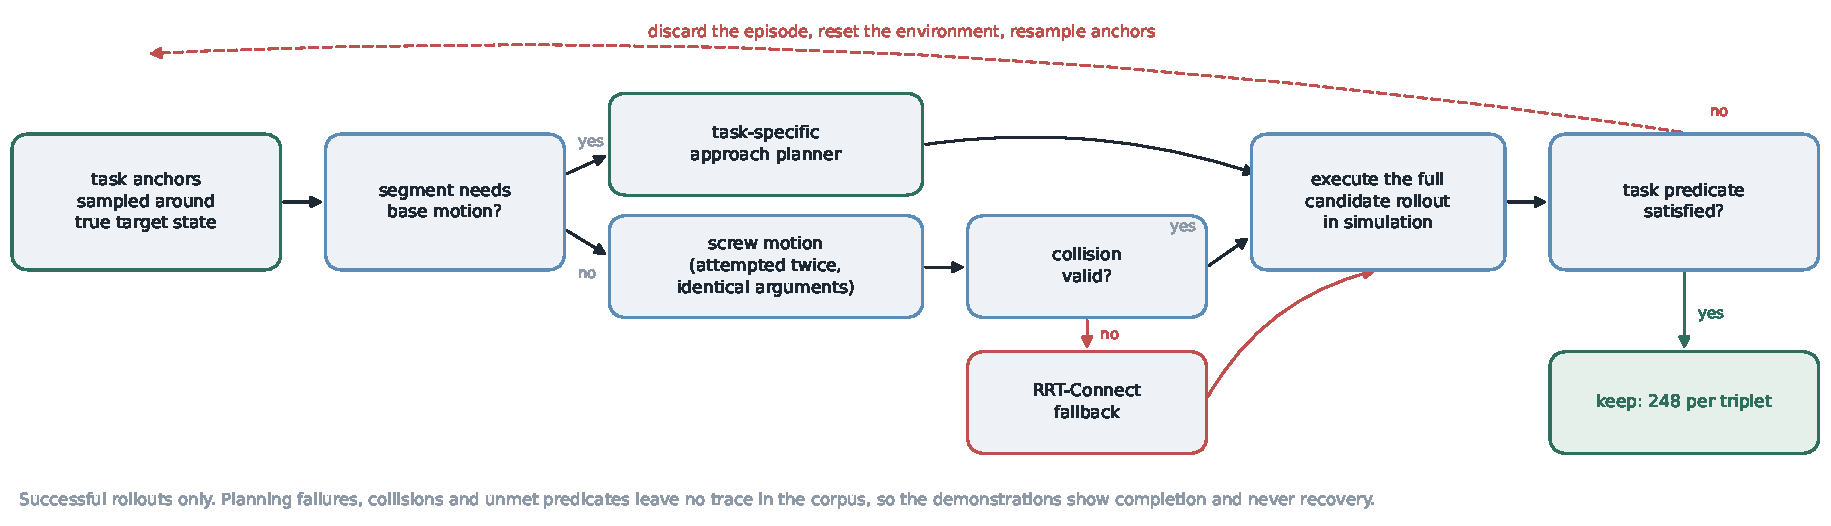
\includegraphics[width=\textwidth]{assets/figures/retail-vla-benchmark/collector_pipeline.pdf}
    \caption{The demonstration collector. Anchors are sampled using privileged object state; each segment is planned by screw motion where the base is fixed and by a task-specific approach planner where it is not; RRT-Connect catches segments that fail collision validation. Only complete rollouts that satisfy the task predicate enter the corpus, and everything else returns to the top of the loop. The two screw attempts are made with identical arguments, so for a deterministic solver the second cannot succeed where the first failed.}
    \label{fig:anchor-sequence}
\end{figure}

Retaining only successful executions produces clean imitation targets and a simple data contract. It also creates selection bias. Demonstrations concentrate on trajectories the planner can solve and omit failed approaches, recovery actions and ambiguous grasps. A learned policy may therefore imitate nominal behaviour without learning how to return to it after a small error. This limitation is revisited when interpreting grasp and pre-grasp failures.

Collected episodes are stored in HDF5 with accompanying metadata, and conversion to other training formats is handled outside the core benchmark. Storage requirements depend on the image encoding, metadata retained and dataset revision; the archived study materials do not support a sufficiently stable size estimate to report one here.

\section{Training protocol}
\label{sec:training}

Octo, SmolVLA, $\pi_0$ and $\pi_{0.5}$ were fine-tuned on a single NVIDIA RTX 4090 using the implementations and configurations recorded in this study. All four use batch size 8, and every run stopped when its preset step counter expired rather than when its loss settled. The comparison that follows is therefore between four fixed-step study configurations, none of which was verified to have converged.

Three of the four use low-rank adaptation. SmolVLA is adapted for 100,000 steps at batch size 8 with rank 64 and $\alpha=64$ on the language expert's query and value projections together with the state and action projections, at a learning rate of $1\times10^{-3}$ decaying by cosine to $1\times10^{-4}$, taking approximately two hours. $\pi_0$ and $\pi_{0.5}$ are adapted for 30,000 steps at batch size 8 with rank 16 on the vision--language backbone and rank 32 on the action expert, applied to the Gemma attention and feed-forward blocks of both, taking approximately two and a half hours each; $\pi_0$ uses AdamW at $2.5\times10^{-5}$ with 1,000 warmup steps and cosine decay to $2.5\times10^{-6}$, while $\pi_{0.5}$ uses $5\times10^{-5}$ with 10,000 warmup steps held constant thereafter, and EMA is disabled for both. Octo is the exception in the recorded study configuration: it is fully fine-tuned for 100,000 steps at batch size 8, also in about two hours, retaining two history observations and a continuous action head.

All four keep an action horizon of 50. Durations are descriptive records from this study, not normalised efficiency comparisons. Step budgets were selected separately for the four implementations under the available hardware rather than matched across models, and no controlled experiment establishes that any one budget was sufficient.

The policies are trained only on atomic tasks. No composite demonstration is used. At evaluation, the oracle issues the next atomic language instruction after the current predicate succeeds. Consequently, any non-zero composite score would demonstrate that an atomic policy can maintain competence across state changes caused by earlier actions. Zero composite performance does not, by itself, reveal whether the problem is long-horizon memory, compounding atomic error or the changed post-action observation distribution.

\section{Evaluation scenarios}
\label{sec:scenarios}

The generator exposes six variation axes: initial robot position, texture, store layout, shelf arrangement, products withheld from a given task and products withheld entirely. The main study combines them into three cumulative conditions, each named for the variable it introduces rather than by an abbreviation.

\textbf{Pose} randomises the robot's start within a task-relevant region and holds everything else at its training value. It tests local robustness to where the robot happens to be standing.

\textbf{Layout} adds new store plans and new floor, wall and ceiling materials. The task and its training products stay familiar; the geometry around them and the visual context do not.

\textbf{Pairing} additionally names a target that was never demonstrated on the evaluated task, though it was demonstrated on another. The shift is compositional rather than perceptual: the product is familiar, the skill is familiar, and only the combination is new. It is therefore a weaker test than one involving a product never encountered anywhere. Section~\ref{sec:verification} explains how the products' presence in the training scenes further limits the claim.

A fourth condition, \textbf{Seeds}, appears only in the per-item tables of Appendix~\ref{app:training-results}. It reruns the stored configurations used to collect the demonstrations and changes nothing at all, which is what makes it useful: it separates imitation of the training distribution from any transfer beyond it.

The software supports unseen shelf arrangements and completely unseen items, yet the headline experiment excludes them. This is a methodological choice based on observed model weakness in simpler settings. It avoids spending most of the evaluation budget on uniformly zero conditions, although it also means the benchmark's most difficult generation capabilities are not validated by the reported baseline table.

Two caveats attach to the definitions above, and both were found after the runs were complete. Layout is realised as described for the three pick-and-place families, whose evaluation scenes come from a seed family disjoint from training. It is not realised as described for the four door tasks, which are evaluated on their own training scenes with only the episode and initial-pose seeds changed, so for those tasks Layout varies texture and starting pose but not geometry. Pairing is realised as described in the sense that its target products were never demonstrated on the evaluated task, but those products stand on the shelves of the training scenes throughout adaptation, which is exactly why the condition is named for the pairing and not for the product. A separate code reading first raised both issues; the author then reproduced them before they were retained. Section~\ref{sec:verification} works through their effect on interpretation.

For each task--item--fixture triplet, 100 trials estimate success. Task-level values in the main table pool the applicable equal-sized triplets. Under Pose and Layout, Basket and Board each pool three triplets, while Floor, Open and Close pool two. Under Pairing, each applicable pick-and-place task pools two held-out product triplets. Door tasks have no meaningful Pairing condition because their instructions never name a product, so those cells are marked not applicable rather than zero. This distinction is essential: zero denotes attempted trials with no successes; not applicable denotes an undefined combination.

\section{Success and side-effect checks}

The task predicate combines goal state, collateral state and robot stability. For a target item $o^*$ and destination region $G$, a simplified pick-and-place predicate can be written as
\begin{equation}
  y=\mathbb{I}[o^*\in G]\,\mathbb{I}[\text{robot static}]\,
  \prod_{o\in\mathcal{N}(o^*)}\mathbb{I}[\Delta(o)\leq\epsilon],
  \label{eq:strict-success}
\end{equation}
where $\Delta(o)$ is non-target displacement, $\epsilon$ is the implementation tolerance and $\mathcal{N}(o^*)$ is the set of non-target products the check actually visits. Both of the last two deserve to be stated rather than left as symbols. The tolerance is 0.1 in position, applied per component together with an equal tolerance on the quaternion, so a neighbour has to shift by roughly ten centimetres before the episode is invalidated. And $\mathcal{N}(o^*)$ is not the whole scene. For the basket task, the evaluator restricts this check to products on the target fixture, which means stock knocked from a neighbouring shelf during the approach goes uncounted. The other pick-and-place tasks range over the scene.

$G$ is likewise more forgiving than the prose suggests. Containment is an axis-aligned box test applied per coordinate rather than a Euclidean distance, so the threshold of 0.2 acts as a half-extent and the accepted region is a cube 0.4~metres on a side; one product uses 0.25. For basket picking that cube is anchored to the robot's own base rather than to a fixed point in the store. Board transfer is tighter, roughly ten centimetres horizontally, with its goal defined as the item's initial position raised by the 0.397~metre clearance between boards. A successful placement is still rejected if surrounding stock moved or the robot has not settled; the thresholds simply describe a looser test than the system chapter originally implied.

Door predicates instead inspect articulation state and stability, which avoids asking a human observer whether a door ``looks open'' but makes the result sensitive to a threshold choice. The showcase requires its named door joint to reach $1.57$~rad within $\pm 0.2$~rad for opening or zero within the same band for closing. The refrigerated fixture is different on both counts: its cover joint has to reach $0.624$~rad, a little under thirty-six degrees, and the tolerance is $\pm 0.1$~rad. Opening a fridge in this benchmark therefore means swinging a door through about two fifths of the arc a showcase door travels, judged twice as strictly. Neither constant is optimal in any principled sense. They are reported so that the numbers in the results chapter can be audited against them.

Mean success is reported as a percentage. Where two conditions can be paired at task level, absolute degradation is
\begin{equation}
  \Delta S_{m,t}=S_{m,t,\mathrm{Pose}}-S_{m,t,\mathrm{Layout}}.
  \label{eq:degradation}
\end{equation}
Absolute percentage-point loss is preferred to a relative percentage for near-zero baselines, where ratios become unstable or undefined.

\section{Failure annotation}

Failed episodes are sampled for qualitative annotation. For each model, approximately ten unsuccessful episodes are drawn from each applicable task--item--fixture combination across Seeds, Pose, Layout and Pairing. The study record reports 2,906 labelled failures. That total does not follow from the procedure just described: the four models and the strata they span imply roughly a hundred and seventy combinations, and 2,906 labels across them averages about seventeen per combination rather than ten. Neither the realised sampling frame nor the episode identifiers were retained with the reported aggregates, so the difference cannot be explained, and neither this total nor the percentages derived from it can be independently re-aggregated from the archived materials. The figure is reported as the study recorded it, and the failure percentages should be read as descriptive of that record rather than as an auditable sample. The annotator records the earliest primary failure visible in the pipeline.

The categories are ordered: \emph{task}, \emph{target}, \emph{move}, \emph{pregrasp}, \emph{grasp}, \emph{drop}, \emph{displace}, \emph{preplace}, \emph{place-coord}, \emph{place} and \emph{partial}. ``Task'' means the behaviour corresponds to another requested operation. ``Target'' means the robot acts on the wrong product. ``Move'' and ``pregrasp'' separate mobile-base approach from local alignment. ``Grasp'' denotes failure to secure the product or handle despite reaching it. The next two categories capture loss of a grasp and disturbance of other products. Placement is divided into approach, coordinate selection and release. ``Partial'' is reserved for incomplete door articulation.

This coding scheme is diagnostic but not perfectly objective. Only unsuccessful episodes are annotated. Labels are assigned manually, and the earliest-failure rule suppresses later consequences. No inter-rater agreement is reported. The distributions should therefore be used to identify large, repeated patterns---for example, grasp accounting for 40\% of $\pi_{0.5}$ failures---rather than to distinguish close percentages as if they were precise sensor measurements.

\section{Validity considerations}
\label{sec:validity}

The controlled parts of the experiment are clear. All four policies receive demonstrations from the same collector, scenes from the same generator and judgements from the same task predicates. The comparison ceases to be matched at adaptation. Each model stops at a preset step count, three use low-rank updates while Octo is fully fine-tuned, and no run is selected by validation performance. Model size, pretraining, optimisation and distance from convergence therefore move together. The table compares four complete study pipelines, not four architectures.

The executed protocol also differs from the written design in several places. A separate reading of the code first raised these discrepancies; the author then reproduced each retained item and classified it as more permissive, more restrictive, or descriptive only. Section~\ref{sec:verification} reports the resulting audit. Unresolved provenance is labelled as such, rather than converted into a directional claim.

Construct validity is narrower than the scale of the generated stores might suggest. The tasks cover cluttered picking, shelf transfer, door articulation and local base positioning. They do not cover store-scale navigation. Every episode begins 1.4~metres from the correct fixture and facing it, with modest translation and yaw perturbations applied on top. The aisles constrain scene geometry and camera context; policies never have to traverse them. Barcode scanning, deformable packaging, people, moving obstacles and damage detection are absent as well.

Control is constrained in two further ways. The policy receives a new observation only after a fifty-action chunk has executed, so it cannot react to contact or pose changes during that interval. Torso lift and head pan are fixed at zero. Conclusions about grasp precision or whole-body reach are conditional on both choices.

External validity remains limited to simulation. The study says nothing direct about sensing noise, friction, compliance, calibration or deformable packaging in a physical store. Statistically, its hundred trials per triplet yield useful point estimates, but the retained task-level aggregates omit episode pairing and layout grouping. They cannot support design-aware condition contrasts. Episode-level outcomes would have allowed paired comparisons, seed-level bootstrap intervals or a mixed-effects treatment of item and layout variation; those records were not preserved in the archived bundle.

\section{Protocol traceability and quality control}
\label{sec:traceability}

Traceability begins with a chain from each reported cell to the checkpoint, code version, scene configuration, prompt and terminal decision that produced it. Seeds alone are insufficient. Layout, arrangement and initial-pose identifiers should be frozen before evaluation, while episode-level outcomes should remain available after aggregation. The present dissertation preserves the reported values and their transformation rules, but not that complete chain.

The same discipline applies at the interface. Camera shape and colour order, proprioceptive fields, action scaling and the ordering of all thirteen commands require explicit checks. Task predicates need positive and negative unit tests at their thresholds. Checkpoint selection should use a validation split, followed by one evaluation on frozen test seeds; repeated attempts, if unavoidable, should be retained.

Failure labels need synchronised views, a written codebook and a second annotator on a stratified subset. Figures and tables should then be generated from the same machine-readable episode records. These steps would turn the next run of this dissertation project from a documented aggregate study into one whose results can be re-analysed without reconstructing lost experimental context.

\endgroup
  % 第四章
\chapter{Results and Discussion}
\label{chap:results}
\begingroup
\justifying
\setlength{\parindent}{2em}
\setlength{\parskip}{0.55\baselineskip}

\section{Reading the results}

Three kinds of evidence appear in this chapter and they answer different questions.

Scene and simulation measurements say whether the generated stores are usable at all---whether a plan can be built, instantiated and stepped quickly enough to run an experiment on. Demonstration and interface results say whether one adaptation pipeline can be laid across four architectures that share almost nothing internally. Policy success rates and failure labels describe the four trained pipelines under the protocol that was actually executed. Only the third body of evidence concerns policy behaviour, and even there the model, adaptation recipe and execution setup remain entangled.

Keeping the three apart matters more than it sounds. A benchmark project can run as designed and still return nothing but low numbers. Those numbers describe the evaluated pipelines, not architecture quality; nor do they prove that every part of the implementation is faultless. Much of this chapter locates that boundary.

\ref{tab:main-results} carries the policy comparison. Every task--item--fixture triplet contains a hundred trials. Under Pose and Layout, Basket and Board pool 300 trials per task-level cell, while Floor, Open and Close pool 200. Under Pairing, each applicable pick-and-place task pools two held-out product triplets, hence 200 trials. A dash marks a condition the door tasks do not have. It is not a zero. The two composite columns are zero for every model and every scenario. One historical $\pi_0$ Pairing aggregate cannot be reconstructed from the archived product-level outcomes and is marked NR rather than treated as a count.

\begin{table}[H]
\centering
\scriptsize
\setlength{\tabcolsep}{2.2pt}
\resizebox{\textwidth}{!}{%
\begin{tabular}{llrrrrrrrr}
\toprule
Model & Scenario & Basket & Floor & Board & Open & Close & Pick 3 & Fridge seq. \\
\midrule
\multirow{3}{*}{Octo}
 & Pose & 1 & 1 & 2 & 3 & 4 & 0 & 0 \\
 & Layout & 2 & 1 & 1 & 2 & 7 & 0 & 0 \\
 & Pairing & 0 & 0 & 0 & -- & -- & 0 & 0 \\
\midrule
\multirow{3}{*}{SmolVLA}
 & Pose & 0 & 0 & 0 & 1 & 2 & 0 & 0 \\
 & Layout & 0 & 0 & 0 & 1 & 2 & 0 & 0 \\
 & Pairing & 0 & 0 & 0 & -- & -- & 0 & 0 \\
\midrule
\multirow{3}{*}{$\pi_0$}
 & Pose & 1 & 1 & 1 & 2 & 2 & 0 & 0 \\
 & Layout & 1 & 1 & 1 & 2 & 2 & 0 & 0 \\
 & Pairing & 0 & NR$^{\dagger}$ & 0 & -- & -- & 0 & 0 \\
\midrule
\multirow{3}{*}{$\pi_{0.5}$}
 & Pose & 1 & 1 & 1 & 2 & 2 & 0 & 0 \\
 & Layout & 1 & 1 & 1 & 1 & 2 & 0 & 0 \\
 & Pairing & 1 & 1 & 3 & -- & -- & 0 & 0 \\
\bottomrule
\end{tabular}}
\caption{Task-level success rates (\%). Every task--item--fixture triplet contains 100 trials. For Pose and Layout, Basket and Board pool three triplets (300 trials), while Floor, Open and Close pool two (200 trials). Pairing pools two held-out product triplets (200 trials) for each applicable pick-and-place task and is undefined for the doors. Successes are summed across equal-sized triplets before division; displayed percentages are rounded to the nearest whole percentage point using round-half-up, while unrounded numerators and denominators govern all calculations. The door-task Layout condition reuses the training plans and changes only texture and starting pose. ``Basket'', ``Floor'' and ``Board'' abbreviate the three pick-and-place tasks. $^{\dagger}$The archived task-level record reports a rounded 1\% for this cell, but the product-level outcomes and unrounded numerator were not retained; it is therefore reported as not recoverable and excluded from count-based calculations.}
\label{tab:main-results}
\end{table}

One thing the table deliberately does not do is collapse. Averaging a door-closing score against a shelf-picking score produces a number, and the number means nothing: the two tasks succeed and fail for unrelated reasons. Reading down a column shows the recorded task-level rates; reading across a row shows the point estimates under each condition. A single overall score would preserve neither distinction.

\section{RQ1: scene generation and computational usability}

RQ1 asked for variation without loss of structure, and on the operational half of that question the pipeline delivers. Different seeds give different store plans rather than reshuffles of one room. Each plan serialises to JSON under a configuration hash, instantiates in ManiSkill3 and keeps its aisles open. Fixtures come out in coherent runs---rows of three to five units placed end to end, with free space between them---rather than scattered across the floor, as \ref{fig:store-generation} shows.

That structure deserves a careful sentence, because the mechanism producing it is coarser than the equations in the system chapter on their own suggest. Every shelf is axis-aligned. What the field decides is where one may sit, not which way it points, and with a decay coefficient of 12 that decision falls to whichever wall or fixture contour happens to lie within about thirty centimetres. The rows are real. They come from a gate applied along a sweep, not from continuous alignment to a smoothly blended orientation.

Product placement contributes controlled visual density but not depletion. The depletion mechanism has no counterpart in the implementation and generated no scene in this study: every shelf in training and evaluation is fully packed. The distinction matters because a designed capability and an exercised one are not the same evidence.

\ref{fig:mesh-performance} records the computational test used for RQ1. Fifty simulation steps were timed on one RTX 4090 while the number of stocked shelving units increased. The original-mesh series rises from 0.21~seconds at one unit to 1.24 at four, where the recorded series ends. The simplified series includes scenes from one to 118 units and remains between 0.23 and 0.42~seconds at the four sampled sizes.

The result is useful but not a matched speed-up estimate. No repeated measurements or original-mesh points above four units were retained, and the 118-unit comparison changes scene size together with mesh detail. At one unit, simplified geometry is actually slower. The defensible conclusion is therefore practical: the recorded setup stepped a densely stocked 118-unit scene with simplified assets, whereas the original-mesh test was not continued beyond four.

\begin{figure}[H]
    \centering
    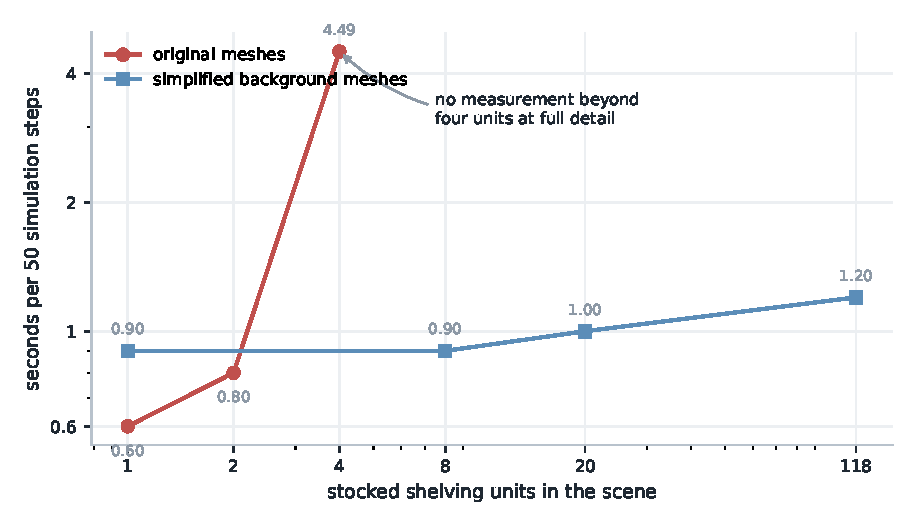
\includegraphics[width=0.68\textwidth]{assets/figures/retail-vla-benchmark/mesh_timing.pdf}
    \caption{Time for 50 simulation steps against the number of stocked shelving units, on log--log axes. The original-mesh series ends at four units, beyond which the scene was impractical to step; the simplified series stays near 0.4~s from one unit to 118. Below roughly two units the original meshes are the faster option, so the two series cross rather than separate.}
    \label{fig:mesh-performance}
\end{figure}

A separate throughput sweep compared state and RGB observations across parallel environments. Its raw result files were not retained, so the apparent saturation of rendered throughput is treated here as a study note, not as a quantitative result. Capacity planning, exact frame-rate claims and memory ratios require the sweep to be rerun from the recorded procedure.

RQ1 is answered for generation and computational cost. Its remaining criteria require narrower conclusions: the scenes were intended to be collision-free, navigable and visually plausible.

Collision-free placement holds by construction, since a candidate that fails the footprint or passage test is never accepted. Visual plausibility was inspected by the author but not measured through a realism study, comparison with surveyed store-plan distributions or physical validation. Navigability was established only as geometric passage provision: the plans leave two metres of clearance and support base motion, but no reported episode required store-scale navigation because each begins 1.4~metres from the relevant fixture. Section~\ref{sec:verification} returns to that limitation.

A generator can therefore be judged sound on the criteria it was built against while leaving the most interesting of those criteria untested. That is the position here.

\section{RQ2: demonstration generation and adaptation}

The collection covers twelve task--item--fixture triplets: 248 successful episodes apiece, 2,976 trajectories and 1,401,169 transitions. It took about ten hours of wall-clock time on a single RTX 4090. Anchor decomposition with screw motion and an RRT-Connect fallback reached that without anyone touching a teleoperation rig, and one observation--action schema then fed four model families whose internals have almost nothing in common. As a supervision source, the pipeline does what it was built to do.

Two things about the corpus are thinner than the totals imply. The layout pool behind it is smaller than the documentation states, because two configuration files meant to generate different stores for board transfer were given the same seed, as were the two for floor recovery; those tasks draw on five distinct plans rather than ten. And the fallback structure is less redundant than the methodology chapter describes---the second screw attempt repeats the first call with identical arguments, which for a deterministic solver cannot change anything. Neither issue costs a result. Both narrow what ``scalable and diverse'' is entitled to mean here.

The more revealing comparison sits in the appendix rather than the main table, and it is the one between Seeds and Pose. Nothing about the scene changes between those two columns. The store is the same store; the shelf holds the same products in the same places; and the instruction is word for word what it was during collection. All that moves is where the robot happens to be standing when the episode starts. The bounds differ by task and neither is large: roughly twenty centimetres of retreat and a quarter of a metre sideways for basket picking, a little under half a metre on both axes for board transfer, with about twenty-two degrees of yaw in either case.

Octo goes from 5\%, 3\% and 3\% on its three board-transfer products to 3\%, 1\% and 1\%. $\pi_{0.5}$ goes from 2\%, 2\% and 2\% on pick-to-basket to 1\%, 1\% and 1\%.

The direction is the one the comparison was built to expose, and the magnitude is too small to build on. Two episodes in a hundred separate Octo's best board-transfer product between Seeds and Pose under a perturbation bounded a little below half a metre on each horizontal axis. In a future convergence-checked run with measurable rates, this comparison would be the sharpest instrument in the chapter, because it needs no argument about what counts as a distribution shift---nothing about the scene changes at all. In the present fixed-step run it is a column of single-digit counts moving by one or two, and it is reported here as a measurement that the protocol supports rather than as a finding the data can carry.

SmolVLA is the one row where the shape survives its own smallness. It records zero on every reported pick-and-place product, in every condition, including the training seeds, while still opening and closing refrigerated and showcase fixtures at rates between 1\% and 4\%. A model that never once places a product in the basket it was shown 248 times, but does occasionally move a door, is not failing uniformly. Whether that pattern would persist under a convergence-checked training configuration is exactly what this study cannot establish.

The present fixed-step configuration does not reveal why this happened. Capacity, pretraining mixture, action normalisation, low-rank adaptation and checkpoint choice remain confounded. At rates this low, success-rate contrasts say little about the underlying model families, even though the failed rollouts still expose where the evaluated pipelines stop.

RQ2 divides cleanly, and the two halves deserve separate answers. On demonstration generation it is answered yes: the pipeline produced 2,976 successful trajectories and 1,401,169 transitions from task specifications without a teleoperation rig, and a single observation--action schema fed four architectures with almost nothing in common. On adaptation it is answered only in the weakest sense available. In the triplet-level Seeds/Pose/Layout table---four models by three modes by twelve task--item--fixture combinations---111 of 144 cells contain at least one success; Pairing and composite-task cells are not included in that count. The four fixed-step configurations nevertheless did not produce dependable behaviour. Because training sufficiency was not established, this study cannot determine whether the corpus suffices for adaptation or isolate the effects of data, compute, optimisation and task difficulty.

Part of the reason is visible in what the collector keeps. It keeps successes, and only successes. The policy learns what a nominal planned trajectory looks like; it receives less evidence about how to correct a base error or reattempt a missed grasp. The prevalence of pre-grasp and grasp failures is consistent with this limitation, although the present experiments do not prove a causal link.

They also do not rule out a competing account, which Section~\ref{sec:failure-modes} returns to. The evaluation client requests a fifty-step action chunk and executes all of it before constructing the next observation, so a policy sees the scene between ten and twenty times across a whole episode and spends the intervening steps committed to a plan it cannot revise. Missing recovery data and missing opportunity to recover produce the same failure label.

\section{RQ3: atomic-task performance}
\label{sec:atomic}

No model achieves dependable task success under the training configuration evaluated here. That sentence is the result, and everything else in this section is an argument about what may and may not be read into it.

The triplet-level Seeds/Pose/Layout table in Appendix~\ref{app:training-results} contains four models, three modes and twelve task--item--fixture combinations: 144 cells in total. Pairing and composite-task cells are not included in that count. The table spans zero to nine successes in a hundred trials, with a mean of 1.5, and 111 cells contain at least one success. The single best cell is Octo closing a showcase door at 9\%. Under Pose, no model exceeds 4\% on any task. The policies are therefore not inert, but the retained outcomes do not support the comparisons this chapter was designed to make.

The limitation on interpretation is stated in Section~\ref{sec:training}. Every model was adapted on one RTX 4090 at batch size 8, for between 30,000 and 100,000 steps, and three of the four through low-rank updates rather than full fine-tuning. No learning-rate or schedule search was carried out. Each run stopped when its preset counter expired, and none was assessed with a validation-based convergence criterion. What \ref{tab:main-results} measures is what these four study pipelines achieved after a few hours of single-card adaptation. That is a legitimate question. It is not the same as asking how well the underlying architectures can learn retail manipulation.

The consequence for interpretation is severe and worth stating in arithmetic rather than in hedging. A hundred trials were run for each item--task--scenario triplet, so a 1\% triplet entry is one successful episode and a 4\% entry is four. The task-level cells pool 200 or 300 trials, depending on scenario and task, and all calculations use the underlying counts rather than the displayed integer percentages. Marginal Wilson intervals could describe uncertainty for an individual pooled rate under an independent-Bernoulli assumption. They are not tests of a model, task or condition contrast, and overlap between two such intervals is not used here as a significance rule. The retained aggregates also omit the episode pairing and grouping needed for design-aware contrasts across shared configurations, items and layouts. Architecture and task rankings are therefore unsupported: adaptation recipes are unmatched, success predicates differ, and item and layout variation has not been modelled.

Three claims a reader may expect from the surrounding literature are worth checking against this table and finding absent. That articulated doors are easier than shelf picking: not supported here---door and pick-and-place columns are separated by two or three episodes. That floor recovery is anomalously hard: not supported---it sits at the floor along with everything else, and under the Seeds condition Octo's highest task mean is in fact floor recovery at 7.5\%. That one policy family transfers better than another: not supported, and Section~\ref{sec:results-shift} explains why the shift comparison cannot be run at all from this baseline. None of the three is refuted by these results; each is simply beyond what they can reach.

One asymmetry is large enough to note without resting anything on it. Octo, the smallest model at 93M parameters and the only one fully fine-tuned rather than adapted through low-rank updates, produces the highest numbers in the table. Whether that reflects the architecture, the smaller parameter count fitting the budget better, or full fine-tuning being the more effective use of a fixed number of steps, this experiment cannot say, since adaptation method and model scale move together across the four rows. It is recorded here as an observation with an experiment attached rather than as a finding.

\section{Distribution shift}
\label{sec:results-shift}

The observed Pose--Layout differences can be calculated from the pooled counts, but they do not answer the transfer question on their own.

The rounded percentages in \ref{tab:main-results} hide several fractional movements, so the comparison has to return to those counts. Ten of the twenty model--task pairs are exactly unchanged from Pose to Layout. Nine move by between one third and two thirds of a percentage point in magnitude. The remaining pair, Octo on door closing, rises from 8/200 to 13/200: five additional episodes, or 2.5 percentage points. Pose success is only 0--4\%, which sharply limits the observable downward range. The retained aggregates also do not permit a design-aware interval for each condition contrast. For the doors, the nominal Layout condition is narrower still because it changes texture and starting pose but not scene geometry.

The distinction between no observed loss and evidence of no loss matters here. A study with a reliable in-domain baseline could estimate a change under a new store plan and attach uncertainty to that contrast. Here the strong floor effect and incomplete statistical record prevent the data from distinguishing a small degradation from no change or improvement. The pick-and-place shift conditions are built and runnable; the door condition does not implement the intended geometric shift. The resulting point differences are reported, but they are not treated as a transfer estimate.

Pairing is the one condition where something is still visible, and only because it is bounded below. Octo and SmolVLA record zero on all three applicable tasks. A historical task-level record gives a rounded 1\% for $\pi_0$ on floor recovery, but the archived product-level outcomes and unrounded numerator were not retained; the cell is therefore marked NR and excluded from count-based comparisons. $\pi_{0.5}$ records 1\% on pick-to-basket, 1\% on floor recovery and 3\% on board transfer; only the board-transfer figure exceeds its corresponding Seeds mean. What can be said is that the two smaller policies reach exact zero when the target product is one they were never asked to handle on that task. That pattern is consistent with a grounding failure, but it is not evidence for one.

Whether current generalist policies transfer across retail-specific geometric and semantic shift remains unanswered in either direction. The study established the conditions, generated the scenes and ran the protocol, but the floor-limited baseline and retained aggregate record do not distinguish a small degradation from no change or improvement. Section~\ref{sec:ablations} sets out the convergence-checked comparison needed before that question can be answered.

One property of the setup remains worth stating because it bounds the question independently of the training budget. It is tempting to explain any Layout effect partly through changed navigation geometry, since the layout moves and the aisles move with it. Episode initialisation sharply limits that reading. The robot is placed 1.4~metres in front of the correct fixture and turned to face it at the start of every episode, in every condition. Basket and Floor then perturb translation by roughly a quarter of a metre per axis; Board uses bounds a little under half a metre; all three use a yaw range of about twenty-two degrees. Nothing in the reported protocol asks a policy to cross a store or to choose between distant fixtures. Even with a budget sufficient to produce measurable rates, the pick-and-place Layout contrast tests visual context and the final approach, not store-scale navigation. The door contrast is narrower again because its geometry does not change.

\section{Composite tasks}

Every composite-task entry is zero. This is the clearest result in the table and the easiest to overstate. The evaluation does not show that a model cannot understand a multi-step natural-language request, because an oracle supplies atomic instructions. It shows that none of the tested adapted policies completed the full execution chain under the protocol.

Compounding atomic error provides a strong baseline explanation. If three stages each succeeded with probability 0.5 and were independent, complete success would be 12.5\%. With a 0.2 atomic rate, it would be 0.8\%. The actual stages are dependent: a poor placement may alter camera views or block the next approach, and the robot state after one completion differs from a clean reset. Zero observed success is therefore compatible with the atomic rates without requiring a separate language-planning failure.

The finding still matters operationally. Retail value comes from finished orders, not isolated benchmark primitives. A policy that occasionally picks one item but cannot sustain a short sequence is not ready for unattended fulfilment.

A column of zeros is also an incomplete account of sequential behaviour. Each composite environment exposes a per-subtask completion flag and a normalised progress count alongside binary success. Those episode-level outputs were not retained in the archived results bundle, so partial progress cannot be reconstructed for this dissertation without rerunning evaluation. The reported result is therefore limited to full-chain completion: no tested pipeline completed either composite task.

\section{Failure modes}
\label{sec:failure-modes}

The aggregate study record reports 2,906 annotated failures. Because the episode-level annotation record was not retained with those aggregates, \ref{tab:failure-share} cannot be independently re-aggregated from the archived study materials and is interpreted descriptively. For Octo, $\pi_0$ and $\pi_{0.5}$, grasping is the largest category at 30\%, 30\% and 40\%. SmolVLA differs descriptively: pre-grasp positioning leads at 40\%, followed by wrong-target interaction at 20\% and grasp at 17\%.

This table retains a descriptive signal even though the success rates sit near the floor, and the reason is structural. Success rates measure how often a policy finishes; failure labels record where sampled unsuccessful executions first stop. A policy that finishes one episode in a hundred still leaves a large pool of failed rollouts from which a structured annotation sample can be drawn. Read the rest of this section on that footing: it describes the interaction between these four trained pipelines and the environment under a constrained adaptation budget, not how capable their architecture families would be with a fuller one.

\begin{table}[H]
\centering
\scriptsize
\resizebox{\textwidth}{!}{%
\begin{tabular}{lrrrrrrrrrrr}
\toprule
Model & task & target & move & pregrasp & grasp & drop & displace & preplace & coord. & place & partial\\
\midrule
Octo & 13 & 22 & 10 & 10 & 30 & 2 & 2 & 1 & 1 & 6 & 3\\
SmolVLA & 9 & 20 & 12 & 40 & 17 & 0 & 0 & 0 & 0 & 0 & 2\\
$\pi_0$ & 3 & 20 & 3 & 20 & 30 & 5 & 1 & 2 & 4 & 5 & 7\\
$\pi_{0.5}$ & 2 & 18 & 1 & 12 & 40 & 4 & 7 & 0 & 2 & 9 & 5\\
\bottomrule
\end{tabular}}
\caption{Share of annotated failures (\%) assigned to each earliest primary category. Rows sum to 100\%.}
\label{tab:failure-share}
\end{table}

Target grounding is the second-largest category for all four models and stays between 18\% and 22\% across them. The benchmark therefore exposes a coupled perception--action problem. A policy can generate plausible movement while acting on the wrong branded product. Since the success predicate checks the named item, visually convincing but semantically incorrect manipulation is rejected.

Movement and pre-grasp labels distinguish two spatial scales. SmolVLA's 12\% movement share and 40\% pre-grasp share indicate breakdown before contact. Octo records 10\% and 10\%, while $\pi_{0.5}$ records 1\% and 12\%. The $\pi$ models more often reach interaction, but reaching the object does not solve the task: 40\% of $\pi_{0.5}$'s labelled failures occur at grasp.

Post-grasp side effects expose a trade. $\pi_{0.5}$ has a 7\% displacement share, higher than the other policies. A model that reaches and interacts more often also creates more opportunities to disturb neighbouring items. Strict side-effect checking is therefore important; otherwise an aggressive shelf sweep could appear as progress.

Before that bottleneck is attributed to the policies, two properties of the evaluation setup deserve to sit next to it, because both bear directly on grasping and neither was visible from the results alone.

The first is the execution horizon. A policy is queried once and returns fifty actions; those fifty actions are executed before it observes anything again. Two fifths of $\pi_{0.5}$'s labelled failures occur at the moment of grasp, after it has already reached the correct product---and a wrist that closes two centimetres off target cannot be corrected until the chunk has run out, whatever the model has learned about correcting it. The demonstration corpus and the execution horizon are two different explanations for the same label, and the experiment reported here does not separate them.

The second is the torso. It does not move. Episode initialisation places the prismatic joint at its lowest position and the evaluation client zeroes the corresponding action element before every step, so vertical reach is fixed for the whole episode in every task. That is worth holding against floor recovery in particular: retrieving an object from the ground and returning it to a shelf above waist height, with a body that cannot rise, is a harder problem than the task name suggests, and it applies to every reported floor-recovery episode. Section~\ref{sec:verification} works through both properties and what they cost.

The next experiments should therefore separate grounding, contact control and recovery data rather than assume that one of them is the bottleneck. The present labels motivate those tests; they do not choose the winner in advance.

\section{Protocol audit against the experimental implementation}
\label{sec:verification}

A fellow student read the implementation against the written protocol and returned a list of possible discrepancies. That reading prompted the audit; it was not an independent replication of the results. I then checked each item against the code and stored configurations. Only discrepancies I could reproduce are reported as confirmed below.

\ref{tab:verification} sets out the confirmed items and what each does to the interpretation of the results.

{\renewcommand{\arraystretch}{1.2}
\begin{table}[H]
\centering
\footnotesize
\begin{tabularx}{\textwidth}{
>{\RaggedRight\arraybackslash}p{0.29\textwidth}
>{\RaggedRight\arraybackslash}X
>{\RaggedRight\arraybackslash}p{0.13\textwidth}}
\toprule
Confirmed discrepancy & What the executed condition actually was & Direction \\
\midrule
Products withheld as targets for a task appear on the shelves of that task's training scenes & The Pairing condition tests a novel task--item combination, not recognition of an unfamiliar product & more permissive \\
The four door tasks reuse their training scenes for the Layout condition & Only texture and starting pose change; layout does not & more permissive \\
The robot starts 1.4~m from the correct fixture, facing it, in every episode & Store-scale navigation is never exercised & more permissive \\
For basket picking, the acceptance region is a $0.4$~m cube and the collateral check covers only products on the target fixture & Completion is more permissive than in the intended scene-wide, task-specific check & more permissive \\
Two pairs of scene configurations share a seed & Board transfer and floor recovery draw on five distinct layouts each, not ten & more permissive \\
The policy observes once per fifty simulator steps & A wrist offset cannot be corrected until the chunk has run & more restrictive \\
Torso lift and head pan are held at zero throughout & Vertical reach is fixed in every task, including floor recovery & more restrictive \\
\bottomrule
\end{tabularx}
\caption{Discrepancies between the documented protocol and the experiment as executed, each reproduced by the author before being accepted. ``Direction'' records whether the executed condition made the test easier or harder than the description implies.}
\label{tab:verification}
\end{table}}

A second group changes the system description rather than a reported score. The tensor field gates axis-aligned placements instead of continuously orienting shelves; layout and arrangement seed sequences are identical in the reported configurations; and the action vector has thirteen elements. Stock depletion and vertical stacking were designed but not implemented. The system chapter now states those boundaries directly.

One item resisted confirmation and is reported as unresolved. The evaluation server for Octo runs with a history length of one, while the training configuration in Appendix~\ref{app:training-results} records two history observations. I was not able to establish which setting produced the reported numbers. Octo's figures therefore carry unresolved evaluation-history provenance; performance need not vary monotonically with history length, so they are neither an upper nor a lower bound on what the checkpoint would achieve under the same budget.

Most confirmed discrepancies made perception or generalisation easier than the written protocol implied. Two made control harder: fifty actions ran between observations, and the torso remained fixed. Their net effect is not recoverable by argument. It needs a rerun.

The audit still removes two tempting interpretations. Door tasks were not exposed to the same geometric shift as pick-and-place, so their apparent robustness cannot be compared. Grasp failures may reflect planner-shaped demonstrations, the open-loop horizon, or both. Composite progress is similarly unresolved because the episode-level subtask outputs were not retained. The only supported composite result is that no pipeline completed a full sequence.

\section{What the benchmark demonstrates}

The dissertation project and the policy study warrant different conclusions. The generator produced structured plans with geometric passage space, and the recorded simplified-mesh setup stepped a 118-unit stocked scene. The collector yielded 2,976 successful trajectories and 1,401,169 transitions; one observation--action schema then served four policy families. These are implementation results. Visual plausibility, store-scale navigation and corpus sufficiency remain untested.

The policy table answers a smaller question. Four fixed-step configurations, adapted on one RTX 4090, did not achieve dependable success. Their Pose baseline was too close to zero, and the retained aggregates too thin, to support model rankings or distribution-shift contrasts. The failure shares remain descriptive because their episode records cannot be re-aggregated; the fifty-step horizon and fixed torso are confirmed properties of the executed protocol, not explanations by themselves.

Whether generalist policies transfer across retail-specific shift therefore remains open. A convergence-checked run, matched conditions and complete episode records are required before this dissertation's evaluation design can answer it.

\section{Implications and a targeted ablation programme}
\label{sec:ablations}

The results suggest a sequence of experiments more useful than immediately adding another model to the leaderboard.

One of them precedes everything else. Until at least one policy is adapted until its in-domain success stops improving, no other ablation in this section can be read, because each of them measures a difference between conditions and there is currently no performance for a condition to change. The cheapest version is one model that fits a single card comfortably, trained with validation-based checkpoint selection until its in-domain success no longer improves and then evaluated under the existing Seeds, Pose, Layout and Pairing conditions. The resulting learning curve and held-out success rate would show whether the preset-step run stopped before measurable performance emerged. If performance remained near zero after that check, separating data, optimisation and task difficulty would require further controlled ablations rather than a single causal attribution.

Two further experiments come directly out of Section~\ref{sec:verification} and should be run alongside it, because until they are, parts of \ref{tab:main-results} cannot be interpreted at all. One is a matched shift for the door tasks: regenerate their evaluation scenes from a seed family disjoint from training, as the pick-and-place tasks already do, and re-measure the Pose-to-Layout loss. At present the door tasks are evaluated on their own training scenes with only texture and starting pose varied, so their Layout column measures something narrower than the pick-and-place columns do. That has to be repaired whatever the training budget, since it is a defect in the protocol rather than in the result. The other is a sweep over the execution horizon. Re-evaluating an unchanged checkpoint at horizons of one, five, ten and fifty costs no retraining, and if grasp failures fall as the horizon shortens then a substantial share of what the taxonomy currently attributes to contact precision belongs to open-loop execution instead.

The remaining ablations concern the policies rather than the scene and evaluation implementation. The first should isolate vision from geometry. Policies could be evaluated on identical layouts with textures changed, identical textures with layouts changed and identical scenes with product pose changed. The present Layout condition combines texture and layout, so any loss it produces cannot be assigned to appearance or to approach geometry. Factorial evaluation would reveal whether augmentation should focus on image statistics, whole-body approach geometry or both.

A second ablation should vary the number and diversity of demonstrations. The configuration used here fixes 248 trajectories per triplet. Training subsets at several sizes would show whether performance is data-limited or whether additional planner-shaped trajectories saturate. Diversity can be changed independently by widening anchor perturbations, varying shelf occupancy and adding more layouts. If twice as many nearly identical successes produce little gain while a smaller diverse set helps, collection effort should shift from volume to coverage.

Recovery data is the next priority. A controlled dataset could perturb the base before pre-grasp, offset the wrist near contact, weaken a grasp or place the object at the edge of the target region. Demonstrations would then show corrective behaviour. Evaluation should measure recovery probability conditional on the perturbation rather than only final task success. This directly tests the hypothesis raised by the failure distribution: policies may know the nominal sequence yet lack a route back after small errors.

Grounding and control should also be separated. One experiment can provide an oracle target mask or 3D target pose while leaving action generation unchanged. If wrong-target errors disappear but grasp remains dominant, perception was only part of the problem. The complementary experiment can retain the policy's target selection but hand the selected object to a privileged grasp planner. The gap between these conditions would quantify the contribution of manipulation precision. Neither oracle represents deployment; both are diagnostic interventions.

Door tasks would make a useful calibration family once any policy performs them reliably enough to compare. Their instruction never names a product, which removes grounding from the picture and leaves articulation and contact as the variables, so controlled changes in handle shape, door mass, friction and required opening distance would map onto performance more directly than they can in the pick-and-place families. Whether closing is genuinely easier than opening---plausible, since closing needs contact while opening needs a handle acquired and held through the swing---is a question the present rates cannot settle.

Composite tasks need richer outputs. Every episode should report the number of completed subtasks, the state at each hand-off and conditional success from stage $k$ to $k+1$. Reset-free continuation can then be compared with an artificial clean reset between atomic stages. If clean-reset composition succeeds while continuous composition does not, state drift and observation change are central. If both remain zero, atomic reliability or instruction switching is sufficient to explain the failure.

Retail-specific pretraining is a plausible response, but it needs a fair test. One model architecture should be pretrained on matched quantities of general manipulation data, synthetic retail data and a mixture. Fine-tuning and evaluation would remain fixed. Such a study could determine whether the retail domain contributes beyond dataset size. The current cross-model table cannot do this because architecture, scale and pretraining mixture all vary together.

Finally, success must be connected to safety and throughput. A policy that completes 60\% of picks but displaces stock in many failures may be less useful than a slower conservative policy. Future reporting could include time to completion, collision impulse, non-target displacement magnitude, recovery count and energy or path length. These are not substitutes for task success. They describe the cost of obtaining it.

This ablation programme follows directly from the benchmark evidence. It treats low scores as a map of unanswered questions, not a verdict that larger models will inevitably solve or fail at retail. The benchmark is most valuable when it narrows the next experiment.

\endgroup
  % 第五章
\chapter{Conclusion and Future Work}
\label{chap:conclusion}
\begingroup
\justifying
\setlength{\parindent}{2em}
\setlength{\parskip}{0.55\baselineskip}

\section{Conclusions}

I set out to run two released RoboBenchMart checkpoints through the benchmark's atomic protocol, using nothing but what is publicly available, and to report what happened. The short answer is that the protocol runs, the results are far from the published ones, and the most likely reason lies in the gap between the checkpoints and the environment they are now evaluated in rather than in the policies as such.

On RQ1, all 42 configurations completed for both Octo and $\pi_{0.5}$, giving 2,520 episodes. Three repairs were needed: an import that an upstream change had removed from the floor environment, the way the client reads instructions through gymnasium wrappers, and per-connection policy state in the Octo server. The evidence that remains is a success flag for each episode, linked to its seed, its log line and its video, with hashes for every file. Per-step trajectories were not saved, because the evaluation script does not ask for them.

On RQ2, the pick-and-place families produced no successes at all, 0 of 900 episodes for each model. The door tasks are the only place where the models differ. $\pi_{0.5}$ closed a door in 37 of 180 episodes and opened one in 2 of 180; Octo closed a door in 4 of 180 and never opened one. Within $\pi_{0.5}$'s closing results, Seeds, Pose and Layout (15, 10 and 12 of 60) are not distinguishable at this sample size. Pairing could not show anything, because the tasks it applies to were already at zero.

On RQ3, the distance from the upstream report is large and systematic. Upstream reports, for example, 82--89\% for $\pi_{0.5}$ on Basket with training seeds, where I observed 0 of 90. Sampling variation cannot produce a gap like that. Since the checkpoints were published, the upstream code has changed the robot's initial joint configuration, the lighting, the robot class and the motion planner, and the demonstration data and scenes have been regenerated; the evaluated release dates from January 2026, the checkpoints from November 2025. I consider this version drift the leading explanation. I have not tested it, and it remains a hypothesis. Several properties of the protocol also bound interpretation regardless of version: door Layout reuses training scenes, every episode starts close to its fixture, actions are executed in open-loop chunks with success read only at chunk boundaries, and the disturbance check covers the whole store.

In plainer terms, the released checkpoints, run on the current benchmark, do not reproduce the published results, and with the records available it is not possible to say exactly why. That is a less satisfying conclusion than a leaderboard. I think it is the more useful one for anyone who intends to use these checkpoints as baselines.

\section{Limitations}

The sample size is the most immediate limitation. Thirty episodes per configuration were enough to establish that pick-and-place rates are low and that $\pi_{0.5}$ closes doors far more often than it opens them, but not enough to resolve differences between conditions of the size the protocol was designed to detect.

The study ran each protocol once. Execution differed between the two models (Octo partly serial and partly on four servers, $\pi_{0.5}$ on one shared server), so the comparison between them is seed-matched but not strictly paired, and run-to-run variation is unmeasured.

The evidence is outcome-level. Without per-step trajectories, and without anyone having watched the videos systematically, I cannot say at which stage failed episodes went wrong. I have deliberately not speculated about failure causes, and the upstream failure taxonomy remains unapplied.

Several facts about the setup are inferred from code rather than observed at run time: the mapping of the locked action indices to the head joints, and the $\pi_{0.5}$ action-chunk length, which the adapter inherits from an OpenPI default I did not check on the revision used. The GPU and several library versions were not recorded during the runs.

Finally, the scope is narrow by design: two checkpoints, atomic tasks only, simulation only. Nothing here speaks to $\pi_0$ or SmolVLA, to composite tasks, or to physical robots.

\section{Future work}
\label{sec:future}

The first experiment I would run is a \textbf{version-aligned re-evaluation}. Check out the upstream code as of early November 2025, pair it with the scene release that preceded the January regeneration (\texttt{demo\_envs} at \texttt{2fd1681a}), and evaluate both checkpoints on a small number of configurations, perhaps two to four, chosen where the upstream and current results differ most, such as $\pi_{0.5}$ Basket and Board under Seeds. Thirty episodes per configuration would be enough. If the rates move close to the upstream figures, the drift hypothesis is confirmed and the individual changes can then be reintroduced one at a time, starting with the initial joint configuration. If they do not, the interface between checkpoint and environment, including action-dimension order and normalisation statistics, is the next place to look.

The second is an \textbf{execution-horizon sweep}. Once a configuration with a non-trivial success rate is available, executing only the first $H \in \{1, 5, 10, 25, 50\}$ actions of each chunk before re-querying the policy would show how much the open-loop execution costs. This needs no retraining. It would also be worth checking the success predicate after every step rather than only at chunk boundaries, which isolates a separate effect.

The third is \textbf{better records}. Running with \texttt{--save-traj} for a subset of configurations would make per-step states available for analysis. With those and the existing videos, the upstream failure taxonomy could be applied under a written coding manual, ideally by more than one annotator, so that failure stages can be reported rather than guessed. Printing the controller's joint list and the policy's action horizon at the start of each run would remove the two remaining inferences.

Only after these steps would it make sense to increase the number of episodes per configuration and revisit the questions the four-condition ladder was designed to answer: how much performance falls from training seeds to new starting poses, to new layouts, and to new task--item pairings.

\section{A staged route to physical validation}

Simulation results, even reproducible ones, are a filter rather than a destination. If a version-aligned baseline is established, a sensible route to physical validation would start with a single shelving unit matching the simulated dimensions, with calibrated cameras placed as in simulation, to separate visual domain shift from contact and controller effects. Real packaging, which is glossy, deformable or transparent in ways the rigid-body simulator does not capture, would come next. Only then would store-scale navigation and safety envelopes around people be worth adding, and reporting would shift from binary success towards measures a store operator cares about, such as items handled per hour, damage to neighbouring stock and the frequency of human intervention.

The step that comes before all of this is less glamorous. A released checkpoint needs a matching, versioned evaluation environment, and the version information has to be recorded at the time the results are produced. The two runs in this dissertation are an attempt to keep such a record.

\endgroup
  % 结论章

% ============================ 参考文献（References） ===========================
% thebibliography管理References
% 选此方式保留references.tex，删除references.bib
% \begingroup
% \renewcommand{\chapter}[2]{}  % 禁止 thebibliography 自动添加目录项
% \endgroup
% \renewcommand{\bibname}{References}
% \input{c-back-matter/references}

% bib格式管理References
% 选此方式保留references.bib，删除references.tex
\renewcommand{\bibname}{References}
\renewcommand\bibsection{\chapter*{\makebox[\textwidth][l]{\bibname}}\addcontentsline{toc}{chapter}{\bibname}}
\bibliographystyle{IEEEtran}             % 指定 IEEE 风格
\bibliography{c-back-matter/references}  % 你的 .bib 文件（不带 .bib 扩展名）

% ============================== 附录（Appendix） ==============================
\appendix
\renewcommand{\thesection}{\Alph{chapter}.\arabic{section}}
\renewcommand{\thefigure}{Figure \Alph{chapter}.\arabic{figure}}
\renewcommand{\thetable}{Table \Alph{chapter}.\arabic{table}}
\chapter{Evaluation Records}
\label{app:details}
\begingroup\justifying
\setlength{\parindent}{2em}\setlength{\parskip}{0.5\baselineskip}

This appendix collects the records behind Chapter~\ref{chap:results}: the result for every configuration, the revisions of every external component, the commands used, and the files in which the raw evidence is kept. All counts were generated from the CSV files in the project repository rather than copied by hand.

\section{Per-configuration results}

Configurations are numbered in the order of \texttt{bash/eval\_model.sh}. The script suffixes map onto the condition names used in this dissertation as \texttt{train} $\to$ Seeds, \texttt{robo} $\to$ Pose, \texttt{uns} $\to$ Layout and \texttt{ood} $\to$ Pairing. The target of \texttt{floor\_beans} is the Heinz baked-beans tin.

{\small
\begin{longtable}{rllcc}
\caption{Successes out of 30 episodes for each of the 42 atomic configurations.}
\label{tab:per-config}\\
\toprule
\# & Configuration & Condition & Octo & $\pi_{0.5}$ \\
\midrule
\endfirsthead
\multicolumn{5}{l}{\small\itshape \thetable\ continued}\\
\toprule
\# & Configuration & Condition & Octo & $\pi_{0.5}$ \\
\midrule
\endhead
\midrule
\endfoot
\bottomrule
\endlastfoot
1 & \texttt{board\_duff} & Seeds & 0/30 & 0/30 \\
2 & \texttt{board\_nestle} & Seeds & 0/30 & 0/30 \\
3 & \texttt{board\_vanish} & Seeds & 0/30 & 0/30 \\
4 & \texttt{open\_fridge} & Seeds & 0/30 & 0/30 \\
5 & \texttt{close\_fridge} & Seeds & 0/30 & 8/30 \\
6 & \texttt{open\_showcase} & Seeds & 0/30 & 0/30 \\
7 & \texttt{close\_showcase} & Seeds & 1/30 & 7/30 \\
8 & \texttt{floor\_beans} & Seeds & 0/30 & 0/30 \\
9 & \texttt{floor\_slam} & Seeds & 0/30 & 0/30 \\
10 & \texttt{basket\_fanta} & Seeds & 0/30 & 0/30 \\
11 & \texttt{basket\_nivea} & Seeds & 0/30 & 0/30 \\
12 & \texttt{basket\_stars} & Seeds & 0/30 & 0/30 \\
\midrule
13 & \texttt{board\_duff} & Pose & 0/30 & 0/30 \\
14 & \texttt{board\_nestle} & Pose & 0/30 & 0/30 \\
15 & \texttt{board\_vanish} & Pose & 0/30 & 0/30 \\
16 & \texttt{open\_fridge} & Pose & 0/30 & 0/30 \\
17 & \texttt{close\_fridge} & Pose & 0/30 & 7/30 \\
18 & \texttt{open\_showcase} & Pose & 0/30 & 1/30 \\
19 & \texttt{close\_showcase} & Pose & 0/30 & 3/30 \\
20 & \texttt{floor\_beans} & Pose & 0/30 & 0/30 \\
21 & \texttt{floor\_slam} & Pose & 0/30 & 0/30 \\
22 & \texttt{basket\_fanta} & Pose & 0/30 & 0/30 \\
23 & \texttt{basket\_nivea} & Pose & 0/30 & 0/30 \\
24 & \texttt{basket\_stars} & Pose & 0/30 & 0/30 \\
\midrule
25 & \texttt{board\_duff} & Layout & 0/30 & 0/30 \\
26 & \texttt{board\_nestle} & Layout & 0/30 & 0/30 \\
27 & \texttt{board\_vanish} & Layout & 0/30 & 0/30 \\
28 & \texttt{open\_fridge} & Layout & 0/30 & 1/30 \\
29 & \texttt{close\_fridge} & Layout & 0/30 & 6/30 \\
30 & \texttt{open\_showcase} & Layout & 0/30 & 0/30 \\
31 & \texttt{close\_showcase} & Layout & 3/30 & 6/30 \\
32 & \texttt{floor\_beans} & Layout & 0/30 & 0/30 \\
33 & \texttt{floor\_slam} & Layout & 0/30 & 0/30 \\
34 & \texttt{basket\_fanta} & Layout & 0/30 & 0/30 \\
35 & \texttt{basket\_nivea} & Layout & 0/30 & 0/30 \\
36 & \texttt{basket\_stars} & Layout & 0/30 & 0/30 \\
\midrule
37 & \texttt{board\_nivea} & Pairing & 0/30 & 0/30 \\
38 & \texttt{board\_fanta} & Pairing & 0/30 & 0/30 \\
39 & \texttt{floor\_fanta} & Pairing & 0/30 & 0/30 \\
40 & \texttt{floor\_duff} & Pairing & 0/30 & 0/30 \\
41 & \texttt{basket\_nestle} & Pairing & 0/30 & 0/30 \\
42 & \texttt{basket\_slam} & Pairing & 0/30 & 0/30 \\
\end{longtable}}

\subsection*{Seeds of the successful episodes}

Every configuration not listed here had no successes. Seeds are those printed on the \texttt{Results:} line of each log and match the video file names.

{\renewcommand{\arraystretch}{1.15}
\begin{table}[H]
\centering
\footnotesize
\begin{tabularx}{\textwidth}{
>{\RaggedRight\arraybackslash}p{0.26\textwidth}
>{\RaggedRight\arraybackslash}p{0.19\textwidth}
>{\RaggedRight\arraybackslash}X}
\toprule
Configuration, condition & Octo & $\pi_{0.5}$ \\
\midrule
\texttt{close\_fridge}, Seeds   & -- & 28, 44, 64, 84, 92, 104, 108, 112 \\
\texttt{close\_showcase}, Seeds & 104 & 12, 16, 36, 60, 76, 84, 132 \\
\texttt{close\_fridge}, Pose    & -- & 28, 32, 52, 64, 84, 92, 96 \\
\texttt{open\_showcase}, Pose   & -- & 32 \\
\texttt{close\_showcase}, Pose  & -- & 0, 76, 128 \\
\texttt{open\_fridge}, Layout   & -- & 42029 \\
\texttt{close\_fridge}, Layout  & -- & 42002, 42013, 42020, 42021, 42024, 42027 \\
\texttt{close\_showcase}, Layout & 42005, 42010, 42019 & 42005, 42010, 42013, 42018, 42019, 42027 \\
\bottomrule
\end{tabularx}
\caption{Seeds of all 43 successful episodes (4 for Octo, 39 for $\pi_{0.5}$).}
\label{tab:success-seeds}
\end{table}}

\subsection*{Wall-clock time per configuration}

Elapsed minutes for each configuration of 30 episodes, from the final progress-bar line of its log. Octo configurations 1 to 17 ran serially and 18 to 42 on four servers in parallel; every $\pi_{0.5}$ configuration ran alongside up to three others on a shared server.

{\small
\begin{longtable}{rllcc}
\caption{Minutes per configuration.}
\label{tab:per-config-time}\\
\toprule
\# & Configuration & Condition & Octo & $\pi_{0.5}$ \\
\midrule
\endfirsthead
\multicolumn{5}{l}{\small\itshape \thetable\ continued}\\
\toprule
\# & Configuration & Condition & Octo & $\pi_{0.5}$ \\
\midrule
\endhead
\midrule
\endfoot
\bottomrule
\endlastfoot
1 & \texttt{board\_duff} & Seeds & 46 & 50 \\
2 & \texttt{board\_nestle} & Seeds & 47 & 50 \\
3 & \texttt{board\_vanish} & Seeds & 41 & 50 \\
4 & \texttt{open\_fridge} & Seeds & 16 & 16 \\
5 & \texttt{close\_fridge} & Seeds & 17 & 13 \\
6 & \texttt{open\_showcase} & Seeds & 93 & 96 \\
7 & \texttt{close\_showcase} & Seeds & 90 & 82 \\
8 & \texttt{floor\_beans} & Seeds & 48 & 48 \\
9 & \texttt{floor\_slam} & Seeds & 50 & 45 \\
10 & \texttt{basket\_fanta} & Seeds & 29 & 31 \\
11 & \texttt{basket\_nivea} & Seeds & 28 & 31 \\
12 & \texttt{basket\_stars} & Seeds & 28 & 32 \\
\midrule
13 & \texttt{board\_duff} & Pose & 43 & 47 \\
14 & \texttt{board\_nestle} & Pose & 46 & 45 \\
15 & \texttt{board\_vanish} & Pose & 46 & 48 \\
16 & \texttt{open\_fridge} & Pose & 15 & 16 \\
17 & \texttt{close\_fridge} & Pose & 14 & 15 \\
18 & \texttt{open\_showcase} & Pose & 90 & 91 \\
19 & \texttt{close\_showcase} & Pose & 92 & 89 \\
20 & \texttt{floor\_beans} & Pose & 44 & 46 \\
21 & \texttt{floor\_slam} & Pose & 45 & 46 \\
22 & \texttt{basket\_fanta} & Pose & 29 & 32 \\
23 & \texttt{basket\_nivea} & Pose & 30 & 33 \\
24 & \texttt{basket\_stars} & Pose & 29 & 31 \\
\midrule
25 & \texttt{board\_duff} & Layout & 43 & 49 \\
26 & \texttt{board\_nestle} & Layout & 44 & 50 \\
27 & \texttt{board\_vanish} & Layout & 45 & 49 \\
28 & \texttt{open\_fridge} & Layout & 18 & 19 \\
29 & \texttt{close\_fridge} & Layout & 15 & 16 \\
30 & \texttt{open\_showcase} & Layout & 92 & 94 \\
31 & \texttt{close\_showcase} & Layout & 88 & 80 \\
32 & \texttt{floor\_beans} & Layout & 46 & 49 \\
33 & \texttt{floor\_slam} & Layout & 45 & 46 \\
34 & \texttt{basket\_fanta} & Layout & 30 & 32 \\
35 & \texttt{basket\_nivea} & Layout & 31 & 32 \\
36 & \texttt{basket\_stars} & Layout & 31 & 32 \\
\midrule
37 & \texttt{board\_nivea} & Pairing & 45 & 48 \\
38 & \texttt{board\_fanta} & Pairing & 46 & 47 \\
39 & \texttt{floor\_fanta} & Pairing & 46 & 46 \\
40 & \texttt{floor\_duff} & Pairing & 47 & 47 \\
41 & \texttt{basket\_nestle} & Pairing & 33 & 32 \\
42 & \texttt{basket\_slam} & Pairing & 31 & 32 \\
\end{longtable}}
The totals are 30.6 hours for Octo and 31.4 hours for $\pi_{0.5}$.

\section{Revisions of external components}

{\renewcommand{\arraystretch}{1.15}
\begin{table}[H]
\centering
\footnotesize
\begin{tabularx}{\textwidth}{
>{\RaggedRight\arraybackslash}p{0.30\textwidth}
>{\RaggedRight\arraybackslash}X
>{\RaggedRight\arraybackslash}p{0.12\textwidth}}
\toprule
Component & Revision & Date \\
\midrule
Octo checkpoint \path{emb-ai/RoboBenchMart_octo} & {\scriptsize\texttt{f3c8de450fc08fb5737d32442a2b1e6ab2993244}}, directory \texttt{1000000} & 2025-11-04 \\
$\pi_{0.5}$ checkpoint \path{emb-ai/RoboBenchMart_pi05} & {\scriptsize\texttt{533ad107347c3568dc2456d1586b665889f0ed18}} & 2025-11-05 \\
Scenes \path{emb-ai/RoboBenchMart_demo_envs} & {\scriptsize\texttt{3dabfaaf9bdf2ba886264a1160dab68ac7043d00}} (``Upload new MP data with regen layouts''); previous revision \texttt{2fd1681a} & 2026-01-22 \\
Benchmark code & upstream \texttt{33ca547} plus my changes (Section~\ref{sec:my-changes}); project HEAD \texttt{4d5e586} & 2026-07-13 (upstream) \\
OpenPI & {\scriptsize\texttt{c23745b5ad24e98f66967ea795a07b2588ed6c79}} plus the RoboBenchMart adapter in \path{scripts/add_rbm.patch}; policy config \texttt{pi05\_eval\_rbm} & -- \\
ManiSkill & 3.0.1, as pinned in the installation guide & -- \\
SAPIEN, mplib, JAX, PyTorch & not recorded at run time & -- \\
GPU & the installation notes record an NVIDIA RTX 4090 (24~GB, driver 570.124.04); the evaluation logs do not record the device & -- \\
\bottomrule
\end{tabularx}
\caption{Revisions of the checkpoints, scenes and software used. Dates for the Hugging Face repositories are commit dates.}
\label{tab:revisions}
\end{table}}

\section{Commands}

The configuration list, scene directories, seeds and step caps are those of \texttt{bash/eval\_model.sh}. For the parallel runs, the commands of that script were split across four worker scripts (\texttt{logs/*\_w0.sh} to \texttt{*\_w3.sh}) without modification of their arguments. A representative client call is

\begin{quote}\small\ttfamily\raggedright
python scripts/eval\_policy\_client.py --host=127.0.0.1 --port=8000 \textbackslash\\
\hspace*{2em}--scene-dir demo\_envs/close\_fridge/ \textbackslash\\
\hspace*{2em}--json-path demo\_envs/close\_fridge/demos/motionplanning/\textbackslash\\
\hspace*{4em}close\_fridge\_248traj\_4workers.json \textbackslash\\
\hspace*{2em}--robot-init-pose-start-seed 10000 --eval-subdir <name> \textbackslash\\
\hspace*{2em}--max-horizon 500 --num-traj 30 --save-video
\end{quote}

The Octo servers were started with \texttt{scripts/octo\_server.py --model-path <checkpoint> --port <8000--8003>}, which builds a policy with one history frame, a predicted horizon of 50 and an execution horizon of 50 for every connection. The $\pi_{0.5}$ server was started from the OpenPI checkout with

\begin{quote}\small\ttfamily\raggedright
XLA\_PYTHON\_CLIENT\_MEM\_FRACTION=0.6 uv run scripts/serve\_policy.py \textbackslash\\
\hspace*{2em}policy:checkpoint --policy.config=pi05\_eval\_rbm \textbackslash\\
\hspace*{2em}--policy.dir=<checkpoint>
\end{quote}

\section{Changes I made to the code}
\label{sec:my-changes}

Compared with upstream commit \texttt{33ca547}, the evaluated code differs in the following files. None changes a success predicate, a scene or a seed.

\begin{itemize}[leftmargin=2em,itemsep=0.15em]
\item \texttt{dsynth/envs/pick\_from\_floor.py}: restored the \texttt{get\_actor\_obb} import removed upstream in \texttt{59ed097}; without it the floor environments raise \texttt{NameError}.
\item \path{scripts/eval_policy_client.py}: read the instruction from \path{env.unwrapped.language_instructions}.
\item \texttt{dsynth/web\_utils.py}: client connections use \texttt{open\_timeout=120} and catch \texttt{TimeoutError}; the server accepts a \texttt{policy\_factory}.
\item \texttt{scripts/octo\_server.py}: one \texttt{Policy} instance, and so one history buffer, per connection.
\item \texttt{scripts/show\_env\_in\_sim.py} and \texttt{tests/test\_overview\_camera.py}: an overview camera for whole-scene recordings.
\item \texttt{docs/INSTALL\_zh.md}: installation and download notes.
\end{itemize}

\section{Logs, artefacts and hashes}

Each result directory (\texttt{results/octo-2026-09-28/} and \texttt{results/pi05-2026-10-02/}) contains four files besides its README:

\begin{itemize}[leftmargin=2em,itemsep=0.15em]
\item \texttt{success\_rates.csv}: one row per configuration with the success count and the log it came from;
\item \texttt{episode\_outcomes.csv}: one row per episode (1,260 per model) with the seed, the success flag, the video path and the source log;
\item \texttt{artifact\_manifest.csv}: path, size and SHA-256 for each of the 1,344 files per model (1,260 MP4, 42 HDF5, 42 JSON);
\item \texttt{log\_manifest.csv}: path, size and SHA-256 for the batch logs, worker scripts and exit-code files.
\end{itemize}

The Octo per-configuration counts come from three serial logs (\texttt{octo\_atomic\_full\_20260927\_021655.log}, seven configurations; \texttt{octo\_atomic\_resume\_20260927\_092850.log}, nine; \texttt{octo\_atomic\_resume2\_20260928\_013647.log}, one) and 25 parallel logs (\texttt{octo\_parallel\_20260928\_021558\_config18.log} to \texttt{config42.log}). The interruption of the second serial log and the deliberate stop of the third are documented in the \texttt{.interrupted} and \texttt{.stopped} files beside them. The $\pi_{0.5}$ counts come from \texttt{pi05\_parallel\_20261002\_105333\_config01.log} to \texttt{config42.log}.

The MP4 and HDF5 files are stored in Git LFS and must be fetched with \texttt{git lfs pull} before the manifests can be checked. The hashes were computed on the evaluation machine when the results were archived; I have not yet re-verified them against a fresh LFS checkout. The JSON files contain no episodes and the HDF5 files are 800 bytes each, because the evaluation script does not pass \texttt{--save-traj}.

\endgroup
 % 附录 B
\input{c-back-matter/appendix-c} % 附录 C

\end{document}
